\documentclass[master=ecws,masteroption=ss]{kulemt}
\usepackage{listings, listings-rust}
\usepackage{bytefield}
\usepackage{color}
\usepackage[usenames,dvipsnames,acmlarge]{xcolor}
\usepackage{pdfpages}

\definecolor{mGreen}{rgb}{0,0.5,0} %very readable shade of green, used by Marco Patrignani in some of his paperss
\lstdefinestyle{custASM}{
  basicstyle=\footnotesize\ttfamily,
  escapeinside={/*@}{@*/},
  mathescape=true,
  commentstyle=\color{mGreen},
  tabsize=4,
  morecomment=[l]{\#},
  numberstyle=\tiny\color{gray},
  numbersep=6pt,
}

\setup{% Remove the "%" on the next line when using UTF-8 character encoding
  inputenc=utf8,
  title={Borrowed Capabilities},
  author={Thijs Vercammen},
  promotor={Prof.\,dr.\,ir.\ D. Devriese\and Prof.\,dr.\,ir.\ F. Piessens},
  assessor={Ir.\ T. Van Strydonck\and Dr. K. Wuyts},
  assistant={Ir.\ T. Van Strydonck}}
% Remove the "%" on the next line for generating the cover page
%\setup{coverpageonly}
% Remove the "%" before the next "\setup" to generate only the first pages
% (e.g., if you are a Word user).
%\setup{frontpagesonly}

% Choose the main text font (e.g., Latin Modern)
\setup{font=lm}

% If you want to include other LaTeX packages, do it here. 

% Finally the hyperref package is used for pdf files.
% This can be commented out for printed versions.
\usepackage[pdfusetitle,colorlinks,plainpages=false]{hyperref}

%%%%%%%
% The lipsum package is used to generate random text.
% You never need this in a real master's thesis text!
\IfFileExists{lipsum.sty}%
 {\usepackage{lipsum}\setlipsumdefault{11-13}}%
 {\newcommand{\lipsum}[1][11-13]{\par And some text: lipsum ##1.\par}}
%%%%%%%

%\includeonly{chap-n}
\begin{document}

\begin{preface}
  I would like to thank everybody who kept me busy the last year,
  especially my promoter and my assistants. I would also like to thank the
  jury for reading the text. My sincere gratitude also goes to my wive and
  the rest of my family.
\end{preface}

\tableofcontents*

\begin{abstract}
  The \texttt{abstract} environment contains a more extensive overview of
  the work. But it should be limited to one page.

  \lipsum[1]
\end{abstract}

% A list of figures and tables is optional
%\listoffigures
%\listoftables
% If you only have a few figures and tables you can use the following instead
\listoffiguresandtables
% The list of symbols is also optional.
% This list must be created manually, e.g., as follows:
\chapter{List of Abbreviations and Symbols}
\section*{Abbreviations}
\begin{flushleft}
  \renewcommand{\arraystretch}{1.1}
  \begin{tabularx}{\textwidth}{@{}p{12mm}X@{}}
    ISA   & Instruction Set Architecture \\
    OBS   & Ownership and Borrow System \\
    PCC   & Program Counter Capability \\
    DDC   & Default Data Capability \\
  \end{tabularx}
\end{flushleft}
\section*{Symbols}
\begin{flushleft}
  \renewcommand{\arraystretch}{1.1}
  \begin{tabularx}{\textwidth}{@{}p{12mm}X@{}}
    42    & ``The Answer to the Ultimate Question of Life, the Universe,
            and Everything'' according to \cite{h2g2} \\
    $c$   & Speed of light \\
    $E$   & Energy \\
    $m$   & Mass \\
    $\pi$ & The number pi \\
  \end{tabularx}
\end{flushleft}

% Now comes the main text
\mainmatter

\chapter{Introduction}
\label{cha:intro}
For many years computer programs have been plagued by vulnerabilities that can be exploited in order to gain control over the execution of a program.
Several classes of these vulnerabilities arise from bugs in the source code and are related to low level control over memory.
Spatial memory issues are vulnerabilities that arise from accessing memory that is outside of the bounds that are supposed to be accessed.
Temporal memory issues on the other hand arise from accessing memory after the reference to that memory is supposed to have been invalidated.
Some famous examples of spatial and temporal memory issues are buffer overflows and use after free whereby an attacker can write to memory that is not supposed to be written to\tomi{add some references whenever you make claims like this; you have very few references atm}.

Over the past decades, several solutions to these issues have been presented and implemented.
One of the most popular solution is the usage of memory safe programming languages that deny the programmer low level access to the memory\tomi{some example refs}.
Instead, the memory is managed by a language runtime and deallocated by a garbage collector.
This solution, however, has a significant performance impact and is thus not applicable to performance sensitive programs such as kernels, browsers and low level system libraries.
These types of programs remain vulnerable and are often a vector for malware to gain control over a system.
A class of devices that are especially vulnerable to these issues are embedded devices, since they have constrained resources and programmers require low level memory management features to gain reasonable performance.
With the advent of the Internet of Things (IoT), these embedded devices are expected to increase in number dramatically\tomi{ref}.

Over the past few years programming languages with strong type systems have gained renewed attention as a way to mitigate these issues and improve security\tomi{strong claim; prove with ref or weaken}.
One of the most popular of these is the Rust programming language\tomi{ref}.
Rust offers a number of security features, but in this thesis we will focus on Rust's ownership and borrowing system.
This system limits what a programmer can do with references to an object in memory, ensuring that memory is always accessed in a safe manner, and statically guaranteeing thread safety.
One of the most important principles of this system is the principle of ``aliasing XOR mutability'' which means that references to a resource in memory are either allowed to mutate the resource or are read-only and can be copied, but not both.
This prevents concurrent write accesses and concurrent read and write access to a resource in memory, which ensures the absence of things like data races.

However, when a Rust program is compiled, it is usually converted into an unsafe assembly language that does not have any of these safety guarantees\tomi{refer to some secure compilation paper}.
This might, for example, open the programs up to attacks on the assembly level if they are linked with libraries that are not written in a programming language with the same safety guarantees.
In this thesis we explore an extension to the capability machine architecture CHERI in order to provide support on the assembly level for the safety guarantees that the Rust programming language offers.

Hardware capabilities are unforgeable pointers that represent authority over a region of memory.
They are comparable to software fat pointers in that they enforce bounds checking and hold permissions that specify how a region of memory can be used.
This model is very effective at combating spatial memory issues, but is less suited to enforce the temporal memory safety guarantees offered by languages with strong type systems.
Nevertheless, CHERI does offer some hardware primitives that software can build upon to strengthen their defense against temporal memory issues.
In this thesis we will add a new type of capability called \textit{borrowed capability}.
This new type of capability is designed to mimic Rust's ownership and borrowing system, but it could be seen in a wider context as an addition to the types of revocation that are already offered by CHERI.

In summary, the goal of this thesis is to design an extension to the CHERI architecture that offers the same memory and thread safety guarantees as the Rust programming language.
\tomi{Mention section numbers in explanation below, since you're going over the sections anyways + update to include discussion section}
To test our design, we will implement it in the Sail specification language, extend the LLVM project to create an assembler for our extension and run test programs on the emulator generated by Sail.
We start off by giving background information about Rust and CHERI as well as information about RISC-V and the Sail language which will be essential for the implementation of our design.
Next, we provide an overview of our design, followed by the details of its implementation in Sail and the details of the LLVM extension.
Finally, we will evaluate our design by constructing a number of assembly example programs and reason about how well they mimic the Rust ownership and borrowing system.

%%% Local Variables: 
%%% mode: latex
%%% TeX-master: "thesis"
%%% End: 

\chapter{Literature Review}
\label{cha:litrev}
The topic of this thesis lies at the intersection of multiple different fields including programming languages, capability machines, formal software verification and instruction set architecture (ISA) design. Understanding this thesis requires background knowledge of each of these individual subjects.

\section{The Rust programming language}
\label{sec:rustbackground}
Rust is a relatively new programming language that aims to provide the high performance associated with other low-level programming languages such as C and C++ while simultaneously preventing a number of classes of bugs related to memory and thread safety that typically arise due to the low-level resource management features necessary to achieve such high performance.
Rust accomplishes this at compile time by statically checking if the source code satisfies the rules of Rust's strong ownership-based type system.
Because these rules are conservative and might reject correct programs, Rust provides an \textit{unsafe} mode in which some of these rules do not need to be satisfied.
Since this thesis is about the safety Rust provides, we only consider \textit{safe} Rust in this section.

\subsection{Ownership}
Central to Rust's resource management model is the concept of ownership.
When a value gets created, ownership of that value will be assigned to a variable.
This value stays valid until its owner goes out of scope after which it cannot be used anymore.
Ownership of a value can be transferred to another variable, when this happens the value cannot be accessed anymore through the original variable.
This is illustrated in listing \ref{code:move} which fails to compile because \textit{a} gets accessed after its value has been moved to \textit{b}.
\begin{lstlisting}[language=Rust,frame=single,caption=Moving a variable,label=code:move]
fn main() {
  let a = String::from("This is a heap allocated string");
  let b = a;
  println!("{}", a);
}
\end{lstlisting}

\subsection{Borrowing}
\label{subsec:borrowing}
As mentioned, Rust follows the principle of ``aliasing XOR mutation'' to prevent a number of bugs related to memory safety and data races.
The borrowing system has a set of rules that enforces this principle.
A value can be borrowed by variables other than its owner, giving those variables temporarily the right to use the value.
There are two types of borrows: a mutable borrow and an immutable (or shared) borrow. 

A mutable borrow allows the borrowing variable to both read and mutate the contents of the value.
To prevent multiple variables mutating the same value at the same time and to prevent variables from reading a value that is being altered, the owner temporarily loses its right to access or lend the value while a mutable borrow is in scope.
As a result, only the borrowing variable is allowed to access the value while a mutable borrow exists.

A shared borrow only allows a borrowing variable to read the contents of the value.
While a shared borrow is in scope, the owner cannot mutate or mutably lend the value anymore.
It is however allowed to read the value and immutably lend the value again.
This means that an unlimited amount of shared borrows can read a value at the same time, but it cannot be mutated while any of those shared borrows exist.

Listing \ref{code:borrowexample} shows a simple program that creates a mutable variable \textit{x}, borrows it mutably and increments the value through that borrow 
Then, after the mutable borrow has ended, the program borrows \textit{x} twice, but this time immutably and uses those borrows to print the value. Note that during the immutable borrow, the owner variable \textit{x} stays available to read from.

\begin{lstlisting}[language=Rust,frame=single,caption=Borrowing an integer,label=code:borrowexample]
fn main() {
  let mut x = 5;
  {
    let m = &mut x;
    *m += 1;
  }
  {
    let s1 = &x;
    let s2 = &x;
    println!("{}, {}, {}",x, s1, s2);
  }
}
\end{lstlisting}

\subsection{Lifetimes}
Section \ref{subsec:borrowing} explained the rules around borrowing, but did not explain how a borrow actually ends.
For this, Rust has a concept called lifetimes.
Every borrow has a lifetime that roughly corresponds to its variable scope which determines when the borrow is valid.
In order to lighten the load on the programmer, the Rust compiler usually implicitly infers the lifetimes of borrows.
However, in some situations it is necessary to explicitly annotate the Rust code with lifetimes.
Listing \ref{code:lifetime_semantics} shows such a situation.
In this example, the function \textit{longest} takes two string references as arguments and returns a reference to one of those.
The function does not know which arguments it will be called with and thus cannot implicitly infer any information about their lifetimes.
This also means it cannot give any guarantees about the lifetime of its return value.
This is why it is necessary to link the arguments to the return value using lifetime parameter annotations.
These annotations allow the function to tell its caller that the returned reference has the same lifetime as the arguments that were passed in.
\begin{lstlisting}[language=Rust,frame=single,caption=Lifetime Example,label=code:lifetime_semantics]
fn main() {
  let string1 = String::from("abcd");
  let string2 = "xyz";

  let result = longest(string1.as_str(), string2);
  println!("The longest string is {}", result);
}

fn longest<'a>(x: &'a str, y: &'a str) -> &'a str {
  if x.len() > y.len() {
    x
  } else {
    y
  }
}
\end{lstlisting} %TODO reference Rust book (this is copied)

\subsection{Semantic Lifetimes}
\label{sec:semantic_lifetimes}
In the previous section we mentioned that lifetimes roughly correspond to scopes.
In reality, Rust's compiler is smart enough to detect the last usage of a variable and ends the lifetime after that last usage.
This means that code like in listing \ref{code:semantic_lifetime} compiles correctly.
Even though the mutable borrow $m$ is still in scope when $x$ gets incremented, the compiler detects that the increment to $m$ is the last usage of $m$ and thus ends its lifetime after that line which allows $x$ to be used again.
In this thesis we will usually place borrows in their own scope when giving examples for clarity reasons.
\begin{lstlisting}[language=Rust,frame=single,caption=Lifetime Example,label=code:semantic_lifetime]
fn main() {
  let mut x = 5;
  let m = &mut x;
  *m += 1;
  x += 1;
}
\end{lstlisting}

\subsection{Borrowing Specifics}
Borrowing has a number of specific interactions depending on the situation and the data types that get borrowed.
Because these interactions are important when we model the Rust semantics on the hardware level, we introduce them in more depth here.

\subsubsection{Reborrowing}
\label{sec:backgroundreborrow}
In section \ref{subsec:borrowing} we stated that a value can not be immutably borrowed while it is mutably borrowed.
This is not entirely accurate as listing \ref{code:reborrow_semantics} shows.
In the example we create a mutable value and borrow it mutably.
We then create a shared borrow from the mutable borrow.
This phenomenon where a borrow gets borrowed again is called a reborrow.
Reborrowing a borrow works similarly to borrowing an owner in the sense that the original borrow --- which we will also call the \textit{parent} --- loses (some of) its permissions while the reborrowed reference --- which we will also call the \textit{child} --- is active.
This can be seen in the difference between listing \ref{code:reborrow_semantics} and listing \ref{code:reborrow_semantics_wrong}.
In listing \ref{code:reborrow_semantics}, the mutable borrow is not used until the lifetime of the shared borrow has already ended and the code compiles correctly.
However, if we move the increment to the value up as in Listing \ref{code:reborrow_semantics_wrong}, the Rust compiler returns an error because the shared borrow still gets used after the increment.
This reborrow feature adds a lot of expressivity to Rust's fairly strict semantics and will have a major impact on our design choices for borrowed capabilities.

\noindent
\begin{tabular}{p{6.65cm} p{6.65cm}}
    \begin{lstlisting}[language=Rust,frame=single,caption=Reborrow Example,label=code:reborrow_semantics]
fn main() {
  let mut x = 5;
  {
    let m = &mut x;
    {
      let s = &(*m);
      println!("{}", s);
    }
    *m += 1;
  }
}
    \end{lstlisting}

    &

    \begin{lstlisting}[language=Rust,frame=single,caption=Wrong Example,label=code:reborrow_semantics_wrong]
fn main() {
  let mut x = 5;
  {
    let m = &mut x;
    {
      let s = &(*m);
      *m += 1;
      println!("{}", s);
    }
  }
}
    \end{lstlisting}
\end{tabular}

\subsubsection{Compound Data Types}
While safe Rust does have a large amount of limitations around slices of data types such as arrays, the borrowing of individual fields of structs is well supported.
This means that it is possible to have multiple mutable references or both mutable and shared references to the same struct at the same as long as they point to different members of the struct.
Listing \ref{code:struct_semantics} shows an example where both fields of a struct get mutably borrowed and independently altered.
This code works and is considered safe Rust.

\begin{lstlisting}[language=Rust,frame=single,caption=Borrowing struct fields,label=code:struct_semantics]
struct S {
  a: i32,
  b: i32
}

fn main() {
  let mut s = S{a: 0, b: 0};
  {
    let a = &mut s.a;
    let b = &mut s.b;
    *a += 1;
    *b += 2;
    println!("{}, {}", a, b);
  }
}
\end{lstlisting}

\subsubsection{Nested References}
\label{sec:rust_nested}
Rust has some complex rules surrounding the loading of references through a borrow that points to a data structure that contains so-called ``nested references''.
In this section we will explain some of these peculiarities through some simple examples.

The first rule pertains to the loading of references through a borrow in general.
Listing \ref{code:nested_move} shows an instantiation \textit{s} of a struct that holds a reference to an integer.
Then, \textit{s} gets borrowed by the variable \textit{b} and the variable \textit{n} tries to load the reference to the integer.
This, however, fails because this code tries to move the reference out of the struct into \textit{n}.
The simple solution to this issue is to borrow the reference to the integer instead, as shown in listing \ref{code:nested_borrow}.
While this may seem like a trivial difference, it is important to note because it means that ownership of a reference cannot be moved out of a struct via a borrow and it means that the variables that have loaded such a reference are bound to a lifetime themselves.
\begin{tabular}{p{6.65cm} p{6.65cm}}
    \begin{lstlisting}[language=Rust,frame=single,caption=Move reference,label=code:nested_move]
struct S<'a> {
  n: &'a mut i32
}

fn main() {
  let mut x= 0;
  let mut s = S{n: &mut x};
  let b = &mut s;
  let n = b.n;
}
    \end{lstlisting}

    &

    \begin{lstlisting}[language=Rust,frame=single,caption=Borrow reference,label=code:nested_borrow]
struct S<'a> {
  n: &'a mut i32
}

fn main() {
  let mut x= 0;
  let mut s = S{n: &mut x};
  let b = &mut s;
  let n = &b.n;
}
    \end{lstlisting}
\end{tabular}

In the next example in listing \ref{code:nested_lifetime} we show some code where the lifetime of this loaded reference is relevant.
In this code we pass the borrow for the struct into the \textit{nested\_borrow} function where it is reborrowed by the \textit{rb} variable.
We then load the integer reference to the variable \textit{n} and try to return \textit{n}.
This fails to compile because the lifetime of \textit{n} is bound to the lifetime of \textit{rb} which does not outlast the function.

\begin{lstlisting}[language=Rust,frame=single,caption=Reborrow Example,label=code:nested_lifetime]
struct S<'a> {
  n: &'a mut i32
}

fn main() {
  let mut x= 0;
  let mut s = S{n: &mut x};
  let b = &mut s;

  let n = nested_borrow(b);
  println!("{}", n);
}

fn nested_borrow<'a>(mut b: &'a mut S) -> &'a i32 {
  *b.n += 1;
  let rb = &mut b;
  let n = &rb.n;
  return n;
}
\end{lstlisting}

Our last example in listing \ref{code:nested_immutmut} shows that \textit{s} is immutably borrowed by \textit{b} and \textit{n} then tries to get a mutable reference through \textit{b}.
This operation, however, fails to compile because Rust does not allow the loading of mutable references through shared references.
The reason for this is that there could be multiple shared references that could be used to load the mutable reference and this behavior would violate the ``aliasing XOR mutation'' principle.
\begin{lstlisting}[language=Rust,frame=single,caption=Mutable reference through shared borrow,label=code:nested_immutmut]
struct S<'a> {
  n: &'a mut i32
}

fn main() {
  let mut x= 0;
  let mut s = S{n: &mut x};
    
  let b = &s;
  let n = &mut b.n;
}
\end{lstlisting}

We will not support all of these rules in our design for borrowed capabilities.

\subsection{Threading}
Thread safety is one of the major features of Rust as exemplified by the Rust slogan ``fearless concurrency''.
In our implementation of borrowed capabilities we will pay attention to safe threading.
Listing \ref{code:thread} shows an example of how threading works in Rust.
We start off by wrapping an integer in the \textit{Arc} construct.
This is necessary because threading in the Rust standard library has no concept of scopes which the Rust borrow checker assumes that created threads outlive their parent thread and thus the values that were owned by the parent even if the programmer correctly waits for the child threads to terminate.
The \textit{Arc} construct works around this by ensuring that a value is not deallocated until each owner of an \textit{Arc} reference is out of scope.
Using a third party threading library with thread scopes would remove the need for the \textit{Arc} construct.
After creating two \textit{Arc} references to the same integer value, we move each one of them into a new thread and then wait for those threads to finish.
Rust ensures that principle of ``aliasing XOR mutation'' is upheld by prevent the mutation of the value inside the \textit{Arc} construct.

\begin{lstlisting}[language=Rust,frame=single,caption=Threading in Rust,label=code:thread]
use std::thread;
use std::sync::Arc;

fn main() {
  let x = Arc::new(5);
  let c = x.clone();

  let handle1 = thread::spawn(move || {
    println!("{}", x);
  });

  let handle2 = thread::spawn(move || {
    println!("{}", c);
  });
  
  handle1.join().unwrap();
  handle2.join().unwrap();
}
\end{lstlisting}

\subsection{Rust Borrow Invariants}
\label{sec:obsinvariants}
In this section we will give a more in-depth explanation of what the Rust safety guarantees are in the form of a set of invariants.
Kan et al. \cite{Kan2018AnEO} identify a set of five invariants that must hold when borrowing in Rust.
These invariants that they refer to as the ownership and borrowing system (OBS) invariants are listed in figure \ref{fig:obsinvariants}.
The OBS invariants ensure that each reference points to a valid block of memory and that each valid block can either be accessed through multiple immutable references or one mutable reference.

\begin{figure}[h]
\centering
\begin{enumerate}
    \item \textit{Unique owner invariant}: Each block has a unique owner.
    \item \textit{Lifetime inclusion invariant}: If $x$ borrows or reborrows $y$ then the lifetime of $x$ should always be within the lifetime of $y$ in order to avoid dangling pointers.
    \item \textit{Lifetime disjoint invariant}: There are \textit{no} two references to the same referent such that their lifetimes intersect and one of them is a mutable reference.
    \item \textit{Writing permission invariant}: If $x$ borrows or reborrows $y$ immutably then the writing permission of $y$ should be disabled until the end of $x$'s lifetime.
    \item \textit{Reading and writing permissions invariant}: If $x$ borrows or reborrows $y$ mutably then both the reading and writing permissions of $y$ should be disabled until the end of $x$'s lifetime.
\end{enumerate}
\caption{The five OBS invariants.\cite{Kan2018AnEO}}
\label{fig:obsinvariants}
\end{figure}

\subsection{Rust Static Guarantees}
Because the compiler automatically deallocates values after their owner goes out of scope, the programmer cannot make typical deallocation related mistakes such as \textit{double free} or \textit{invalid free}.
An owner can only go out of scope when no more borrows exist, meaning that a \textit{use after free} bug is impossible.
The borrow system eliminates the necessity of using raw pointers and prevents problems relating to null pointers or buggy pointer arithmetic.
Rust also prevents simultaneous read and write access to a value, making data races impossible.
All of these static safety guarantees also result in Rust's ability to prevent thread related bugs and enforce thread safety.

%TODO ref rustbelt and rust book

\section{CHERI}
Capability Hardware Enhanced RISC Instructions (CHERI) is an architecture neutral model of hardware supported capability machines, largely developed by researchers at Cambridge University.\cite{UCAM-CL-TR-951} This chapter starts off with a general introduction to capabilities which is followed by a deeper look into the specifics of the CHERI protection model and its implementation in the RISC-V ISA.

\subsection{Capabilities}
\label{sec:capintro}
Capabilities are unforgeable tokens that give a process access to some resource. They are created by a privileged entity such as the hardware or the kernel. This privileged entity also checks and enforces the correct use of capabilities. In the context of memory they are a method of addressing memory that is different from the traditional approach of using raw integer pointers. Owning a memory capability gives a process the rights to read from, write to or execute the contents of a location in memory, depending on the access permissions of the capability. Memory capabilities can usually give access to a range of memory locations which allows them to properly express concepts like arrays and structs. Figure \ref{fig:capability} depicts a capability layout from an early iteration of the CHERI design and allows for a simple explanation of how capabilities work.

\begin{figure}[h]
\centering
\definecolor{lightgray}{gray}{0.8}
\begin{bytefield}[endianness=big, bitwidth=.55em]{64}
    \bitheader{0,63} \\
    \bitbox{8}{\color{lightgray}\rule{\width}{\height}} & \bitbox{24}{\textbf{otype} (24 bits)} & \bitbox{31}{\textbf{permissions} (31 bits)} & \bitbox{1}{\textbf{s}} \\
    \bitbox{64}{\textbf{offset} (64 bits)} \\
    \bitbox{64}{\textbf{base} (64 bits)} \\
    \bitbox{64}{\textbf{length} (64 bits)}
\end{bytefield}
\caption{An old version of the CHERI capability layout.\cite{Watson2015CHERIAH}}
\label{fig:capability}
\end{figure}

A process that holds a capability like in figure \ref{fig:capability} is able to access the memory locations between \textit{base} and \textit{base+length} by modifying the \textit{offset} so that \textit{base+offset} points to the desired memory address. The process can freely modify the \textit{offset} field, but it is only allowed to alter the \textit{base} or \textit{length} fields in such a way that they point to a subset of the memory that the current capability points to. If the process tries to dereference the capability when the \textit{offset} field is set in such a way that it does not point to a memory location within the permissible range, some sort of error will be raised, such as a hardware exception in the case of CHERI. This prevents a whole range of possible security issues that are present in systems using raw pointers such as faulty pointer arithmetic and buffer overflows.

The \textit{permissions} field contains a bitmap of various permissions such as read, write and execute. Modifying the \textit{permissions} field works similar to modifying the \textit{base} and \textit{length} fields in the sense that the process can only modify them in such a way that results in less permissions than the current capability. This form of monotonicity where a process can only reduce the rights on the capability it holds is central to the CHERI design. It gives a process a method to efficiently restrict the rights on the capabilities it delegates to components it may not trust while still retaining those rights for itself (by holding a copy of the original capability). The \textit{otype} and \textit{sealed} (\textit{s}) fields will be explained in section \ref{sec:sealed}.

\subsection{CHERI Capability Layout}
\label{sec:cheri_cap_layout}
Figure \ref{fig:cheri_capability} shows the layout of 128-bit capabilities in the latest iteration of the CHERI specification. This capability format is intended for use in 64-bit architectures. While a 64-bit capability format intended for use in 32-bit architectures exists, this format is too limited to support the work in this thesis, so we will not consider it here.

\begin{figure}[h]
\centering
\definecolor{lightgray}{gray}{0.8}
\begin{bytefield}[endianness=big, bitwidth=.55em]{64}
    \bitheader{0,63} \\
    \bitbox{14}{\textit{p}'16} & \bitbox{3}{\color{lightgray}\rule{\width}{\height}} & \bitbox{16}{otype'18} & \bitbox{3}{\textit{$I_E$}} & \bitbox{8}{\textit{T}[11:3]} & \bitbox{5}{\textit{$T_E$}'3} & \bitbox{10}{\textit{B}[13:3]} & \bitbox{5}{\textit{$B_E$}'3} \\
    \bitbox{64}{\textit{a}'64}
\end{bytefield}
\caption{The current iteration of the CHERI capability layout.\cite{UCAM-CL-TR-951}}
\label{fig:cheri_capability}
\end{figure}

These capabilities consist of two 64-bit words with a number of fields:

\begin{itemize}
    \item p: The permissions field is a bitvector containing various permissions, explained in more detail in section \ref{sec:capperms}. It consists of two subfields:
        \begin{itemize}
            \item hperms: The hardware permissions field is 12 bits wide and contains the permissions defined by CHERI such as read, write, execute and various others.
            \item uperms: The user permissions field is 4 bits wide and is reserved for application specific uses.
        \end{itemize}
    \item reserved: There are 3 unused bits reserved for possible future or implementation specific use.
    \item otype: The object type field is used by sealed capabilities as explained in section \ref{sec:sealed}.
    \item bounds: The next 27 bits are used to define the bounds of the capability. This is a compressed representation of the \textit{base} and \textit{length} fields described in section \ref{sec:capintro}. The bounds bits are explained in more detail in section \ref{sec:bounds}.
        \begin{itemize}
            \item $I_E$: the internal exponent.
            \item E: the exponent.
            \item T: the top.
            \item B: the base.
        \end{itemize}
    \item a: The address field holds the referenced memory location. This field is similar to a raw integer pointer.
\end{itemize}

\subsection{Capability Tags}
In CHERI, each register and each capability-aligned memory location is associated with a 1-bit tag that is kept out of band. This means that the tag cannot be directly accessed by the software. A tag indicates the presence of a valid capability and is read from and written to in certain hardware operations. The tag allows the hardware to guarantee that the software does not alter its capabilities in a way that is not allowed. In general, if a program wants to alter a capability in any way, it needs to do this through CHERI capability manipulation instructions. If the program writes to a memory location or register where a capability resides using traditional write instructions, the hardware will clear the tag which invalidates the associated capability. It is then no longer considered a valid capability and it cannot be used anymore by the majority of CHERI instructions. It is the responsibility of the compiler to ensure that no necessary capabilities are accidentally invalidated. 

\subsection{PCC \& DDC}
Two of the most important special registers added by CHERI are the program counter capability (PCC) and the default data capability (DDC). The PCC extends the traditional program counter as a capability which allows applications to the fetching\tomi{sentence is off} of instructions to memory locations for which the application holds a capability with execute permissions.

The DDC register holds a capability through which traditional, non-capability memory accesses are indirected. This is a hybridization feature that allows for running non-CHERI compiled binaries on a CHERI CPU with some of the CHERI safety guarantees. Every legacy load or store instruction is checked against the bounds and permissions of the capability in the DDC register. If the memory access is allowed by the capability in the DDC register, the instruction completes successfully. If however the memory access is not allowed, the instruction that is attempting to access memory will trap.

\subsection{Capability Permissions}
\label{sec:capperms}
The permissions field is a simple bitvector where each bit corresponds to a certain permission. An application can manipulate permissions on their capabilities through the \textit{CAndPerm} instruction. The \textit{CAndPerm} instruction takes a capability and a bitmask as arguments and outputs a capability with that bitmask applied to the permissions field. This operation ensures that an application cannot give itself more permissions since a bitmask can not be used to set a bit that was not originally set. This means that the capability rights monotonicity is preserved.

The hardware permissions (\textit{hperms}) subfield is a 12-bit field that contains the permissions that are interpreted by the hardware. Given below is the interpretation of each bit in the vector, starting from the least significant bit. The \textit{Global} and \textit{Permit\_Store\_Local\_Capability} permissions are further explained in section \ref{sec:global}. The \textit{Permit\_Seal}, \textit{Permit\_CInvoke} and \textit{Permit\_Unseal} permissions are further explained in section \ref{sec:sealed}.
\begin{itemize}
    \item Global: Allow this capability to be stored by all capabilities that have the \textit{Permit\_Store\_Capability} permission.
    \item Permit\_Execute: Allow this capability to be used to fetch instructions.
    \item Permit\_Load: Allow this capability to be used to load data from memory.
    \item Permit\_Store: Allow this capability to be used to store data in memory.
    \item Permit\_Load\_Capability: Allow this capability to be used to load capabilities from memory. The \textit{Permit\_Load} bit is also required.
    \item Permit\_Store\_Capability: Allow this capability to be used to store capabilities in memory. The \textit{Permit\_Store} bit is also required.
    \item Permit\_Store\_Local\_Capability: Allow this capability to be used to store capabilities that do not have the \textit{Global} bit set. The \textit{Permit\_Store} and \textit{Permit\_Store\_Capability} bits are also required.
    \item Permit\_Seal: Allow this capability to be used to seal other capabilities.
    \item Permit\_CInvoke: Allow this capability to be used as an argument to CInvoke.
    \item Permit\_Unseal: Allow this capability to be used to unseal other capabilities.
    \item Permit\_Set\_CID: Allow this capability to be used to set the architectural compartment ID.
    \item Access\_System\_Registers: Allow this capability to be used to access privileged registers. The interpretation of this bit is architecture-specific.
\end{itemize}
The 4-bit user permissions field (\textit{uperms}) is intended for application specific use and is not interpreted by the hardware. These bits follow the same principles as the \textit{hperms} bits, but an application can give its own semantic meaning to them.

\subsection{Global and Local Capabilities}
\label{sec:global}
A capability can either be \textit{global}, which means it can be stored in memory by any capability that has the \textit{Permit\_Store\_Capability} permission, or \textit{local}, which means it can only be stored by capabilities that have the \textit{Permit\_Store\_Local\_Capability} permission. These low level permissions can be used to construct higher level restrictions on the propagation of capabilities depending on which capabilities have the \textit{Global} and \textit{Permit\_Store\_Local\_Capability} bits set. This propagation restriction depends on different components of software having access to different parts of memory and having access to capabilities with differing \textit{Permit\_Store\_Local\_Capability} permissions.

For example, if a component has exclusive access to some piece of memory (i.e. no other component has a capability pointing to that part of memory) through a capability with \textit{Permit\_Store\_Local\_Capability} and it has no other capabilities with \textit{Permit\_Store\_Local\_Capability}, it means that \textit{local} capabilities cannot be passed on to other components. As another example, consider a component that has a capability pointing to a shared part of memory with \textit{Permit\_Store\_Local\_Capability}. This means that the component can store \textit{local} capabilities to that shared part of memory. Other components can then load the \textit{local} capability from the shared memory, but they cannot store it again, unless they have a capability with \textit{Permit\_Store\_Local\_Capability} themselves.

%TODO: make it more clear that the following examples are copied
Some possible applications for this system are restricting local stack capabilities to be stored only on the local stack or letting capabilities flow in only one way through a shared buffer.\cite{UCAM-CL-TR-951} %page 59

\subsection{Linear Capabilities}
%TODO: this is probably a bit too brief
Linear capabilities is a concept that has been proposed by multiple researchers and is currently being considered for adoption in CHERI. We briefly introduce it here because the work in this thesis makes extensive use of linear capabilities. Linear capabilities are capabilities that can not be copied in any way.\tomi{Intuitively explain why this is useful, and what guarantees you get from this}. Linear capabilities can be used to enforce well-bracketed control flow and local state encapsulation \cite{10.1145/3290332}.

Two proposed instructions that relate to the splitting and merging of linear capabilities with congruent sections of memory have been found to be difficult to implement in microarchitecture because they have to write to two different registers in the same instruction. For the work in this thesis we rely on these instructions. We acknowledge these difficulties as a weakness in our design, but do not attempt to mitigate these issues.

\subsection{Revocation}
Capabilities are particularly well suited to ensure spatial memory safety, but they are not inherently designed to solve temporal memory safety issues.
One important concept in preventing temporal memory safety issues is \textit{revocation}; repealing the access an untrusted stakeholder has to a certain resource.
Prior work has attempted to solve the revocation issue in several ways.
CHERIvoke \cite{xia_cherivoke_2019} and Cornucopia \cite{nathaniel_wesley_filardo_cornucopia_2020} present a method of revoking capabilities by modifying the system's memory allocator and periodically sweeping memory to remove capabilities pointing to memory that has been freed.
While this approach to temporal safety could be tailored to different scenarios than just memory allocation, it includes the memory allocator into the trusted computing base (TCB), and could be prohibitively expensive if the memory sweep is required often (e.g.\ after each call to an adversary).
Two other approaches each use \textit{local} and \textit{linear} capabilities to implement a type of revocation that does not rely on a memory sweep or a software TCB, and could perform better in the aforementioned scenarios.

Skorstengaard et al.\ introduce a new calling convention using local capabilities \cite{skorstengaard:esop18} to enforce revocation on the stack.
Georges et al. have proposed a new type of capability, called uninitialized capabilities \cite{georges_efficient_2021} to prevent the necessity of clearing the write-local memory in this stack setting.
Van Strydonck et al.\ used linear capabilities to implement revocation in a fully abstract compiler from separation-logic-verified C code to a capability machine \cite{van_strydonck_linear_2019}, and Skorstengaard et al.\ used them to enforce well-bracketed control flow and stack encapsulation \cite{skorstengaard:popl19}.
Because linear capabilities cannot be copied at all, they are a very restrictive way of revoking capabilities.
For example, they cannot be used to provide multiple parties with simultaneous read-only access, or in a multi-threaded setting.

Our design of borrowed capabilities will provide a new way of revocation which we will discuss in more depth in chapter \ref{chap:discussion}.

\subsection{Sealed Capabilities}
\label{sec:sealed}
In their most basic form, sealed capabilities are capabilities that cannot be modified or dereferenced. Normal unsealed capabilities are identified by an otype value of $2^{18} - 1$; for all other values of the 18-bit \textit{otype} field, the capability is considered sealed. CHERI currently reserves 16 otype values for specific interpretations, all other otype values can be used for code-data pairs, further explained below. The reserved otype values range from $2^{18} - 1$ to $2^{18} - 16$.The first of these values is used for unsealed capabilities, as mentioned above. The second one is used for sealed entry (sentry) capabilities, the other values in the range have currently not been assigned. Sentry capabilities are intended to be used as pointers to code that can be executed and jumped to by control flow instructions. The modification restriction of sealed capabilities fits this use case well because it prevents applications from creating unintended control flows.

The main use case for sealed capabilities and the \textit{otype} field is the concept of code-data pairs. Code-data pairs are designed to support compartmentalization of software within a single address space. As their name implies, a code-data pair is a pair of two capabilities, one of them pointing to the code of a compartment and the other pointing to the data used by this compartment. Code-data pairs are a form of object capabilities which are essentially closures: encapsulated objects that contain code to execute and an environment, represented by the code and the data capability respectively.

Code-data pairs are created by sealing both capabilities with the CSeal instruction. This instruction takes two input operands. The first one is the code or data capability to be sealed and needs to have the \textit{Permit\_CInvoke} permission. The second one is a capability with the \textit{Permit\_Seal} permission. CSeal sets the otype field on the code or data capability to the value in the address field of the second operand. Two capabilities with the same otype value are considered code-data pairs and can be used as input operands of the CInvoke instruction. The CInvoke instruction unseals the code-data pair, moves the code capability to the PCC and places the data capability in a predetermined register.

This system can be used as a security domain transition between two mutually distrusting compartments. The caller cannot tamper with the callee since the references it holds to the callee --- the code-data pair --- are sealed and the callee cannot access any of its caller's state, except for the arguments that the caller passed through CPU registers.

\subsection{Capability Bounds}
\label{sec:bounds}
While the full calculations behind the bounds of a capability are outside of the scope of this thesis, we will explain the general principle behind them in this section. The $I_E$ field is a bit to indicate whether the \textit{E} field is used. When $I_E$ is equal to zero, the size of the \textit{E} field is 0 and $T_E$ and $B_E$ are part of the \textit{T} and \textit{B} fields respectively. If $I_E$ is equal to one, $T_E$ and $B_E$ are joined together to form the \textit{E} field with a size of 6 bits, shortening the \textit{T} and \textit{B} fields in return. These bits that are in this case missing from \textit{T} and \textit{B} are considered to be zeros.

The \textit{B} and \textit{T} fields are used in the calculation of the base and top values --- the addresses which \textit{a} must lie between. The $50 - E$ most significant bits of the base and top are copied from the \textit{a} value, possibly incremented or decremented with a correction value. This correction value is calculated from various comparisons between certain bits of the \textit{T}, \textit{B} and \textit{a} fields. The next 14 bits of the base value are directly copied from the \textit{B} field. The next 14 bits of the top value are copied from the \textit{T} field, extended with 2 bits, based on the \textit{B} and $I_E$ field. The remaining \textit{E} bits are zeros. This means that using the \textit{E} field by setting the $I_E$ bit increases the representable range to potentially the entire address space at the cost of accuracy, introducing alignment requirements. The accuracy cost is inversely proportional to the size of the \textit{E} value.

\subsection{Capability Exceptions}
In general, when an application does something that is not allowed, such as dereferencing a memory location without the proper permissions or modifying a sealed capability, the hardware will raise an exception and will transfer execution to the appropriate exception handler. This allows an operating system to handle the exception in a correct manner.

\subsection{RISC-V Implementation}
\label{sec:cheri-risc-v}
While an implementation of CHERI in MIPS exists, in this thesis we work with the RISC-V implementation of CHERI so we will restrict this section to RISC-V and to the parts of CHERI-RISC-V that are relevant to this thesis. CHERI-RISC-V is an extension of the RISC-V instruction set that implements the CHERI protection model. CHERI-RISC-V uses instructions space that is reserved for extensions in the RISC-V instruction set. This instruction space differs depending on whether compressed RISC-V instructions are used or not. CHERI-RISC-V supports both compressed and non-compressed instructions, but makes some changes for compressed instructions to account for the reduced opcode space.

CHERI-RISC-V supports both a split and a merged register file. With a split register file, registers able to hold capabilities are separate from the integer registers. In contrast, with a merged register file all registers are able to hold both capabilities and integers where the upper 64 bits of a register are ignored if an operand register is interpreted as an integer. A merged register file has significant performance benefits. In this thesis we will work with a merged register file.

Capabilities in CHERI-RISC-V have an extra 1-bit field used for the encoding-mode flag. The addition of this flag reduces the amount of reserved bits from three to two. The encoding-mode flag is used on capabilities that are used as the PCC. When the bit is off, the system is in integer encoding mode, meaning that operands to traditional RISC-V loads and store instructions are interpreted as traditional integer addresses. When the bit is set, the system is in capability encoding mode, meaning that operands to traditional RISC-V load and store instructions are interpreted as capabilities. The big advantage of this mode is that traditional RISC-V load and store instructions can be used with capabilities, saving a significant amount of opcode space.

%%% Local Variables:
%%% mode: latex
%%% TeX-master: "../thesis"
%%% End:

%\section{RISC-V \& SAIL}
RISC-V is an open RISC ISA created by researchers at Berkeley University \cite{Waterman:EECS-2011-62}. Its open nature has made it a popular ISA for education and research purposes with a large amount of available tooling. In this thesis we use CHERI's extension of the RISC-V ISA, called CHERI-RISC-V.

\subsection{Instruction layout}
\label{sec:riscvenc}
RISC-V offers multiple instruction types that differ in the way their bits are interpreted.
In this thesis we will only use R-type instructions, shown in figure \ref{fig:rtypeinst}.

\begin{figure}[h]
\centering
\definecolor{lightgray}{gray}{0.8}
\begin{bytefield}[endianness=big, bitwidth=1em]{32}
    \bitheader{32,25,24,20,19,15,14,12,11,7,6,0} \\
    \bitbox{7}{funct7} & \bitbox{5}{rs2} & \bitbox{5}{rs1} & \bitbox{3}{funct3} & \bitbox{5}{rd} & \bitbox{7}{opcode} \\
\end{bytefield}
\caption{R-type RISC-V instruction.}
\label{fig:rtypeinst}
\end{figure}

An R-type instruction consists of 6 different fields, each with their own meaning. The operation code (\textit{opcode}) field is 7 bits wide and specifies the class of instructions to be used. All of the instructions introduced in this thesis will use the CHERI-specific opcode of \textit{1011011} which is one of the opcodes that RISC-V reserves for extension usage. The exact instruction to execute is further indicated by the \textit{funct3} and \textit{funct7} fields which are 3 and 7 bits wide respectively. The other three fields, \textit{rd}, \textit{rs1} and \textit{rs2} specify which registers should be used in the instruction. \textit{rd} indicates the destination register while \textit{rs1} and \textit{rs2} indicate the first and second source registers.
In CHERI, the \textit{rs2} field is also used as an extra funct field for some instructions, called \textit{funct5}.
This is the case for instructions that use only one source register and a destination register.
Because CHERI has a distinction between integer and capability registers, CHERI introduces the \textit{cd}, \textit{cs1} and \textit{cs2} notation.
The \textit{c} registers refer to capability registers while \textit{r} registers refer to integer registers.
This distinction is merely cosmetical as the underlying bits just represent a register number and are agnostic to whether the field is interpreted as an integer or capability register.

\subsection{Registers}
The base RISC-V ISA provides 32 integer registers that are named by an x in front of their number.
Reading from the \textit{x0} register always results in reading zero, regardless of what was written to the register.
This means that writing to \textit{x0} has no effect and can be used as a no-operation (NOP).

CHERI-RISC-V introduces another 32 capability registers, named \textit{c0} through \textit{c31} which may or may not be shared with the integer registers.
As mentioned before, in this thesis we work with a shared register file which means that there are only 32 registers and each register can be interpreted as an integer or as a capability register.
Like \textit{x0}, \textit{c0} contains a fixed value which is called the null capability, which has most of its fields set to zero.

%TODO explain opcodes used in our examples?

\subsection{LLVM}
\label{sec:llvm_background}
While several compilers that target RISC-V exist, the only compiler that targets CHERI-RISC-V is CHERI's fork of the LLVM project \cite{cherillvm}.
The LLVM project offers a large amount of tools related to compiling such as a compiler for several programming languages, a linker, an assembler, a disassembler and much more.
In this thesis we will extend CHERI's fork of the LLVM project to support the new instructions we introduce and we will use LLVM's assembler to turn assembly source files into executable binary files.

The code snippet in figure \ref{fig:insttemplate} shows the instruction definition for the CHERI function \textit{CGetPerm} and the template used by that definition.
The template accepts a 5 bit argument \textit{funct5}, a string with the instruction name and an indication whether the used registers are integer or capability register for which defaults are provided.
These arguments are then mapped to an R-type instruction with a fixed \textit{funct7} field of 0x7f, an \textit{rs2} field with the provided \textit{funct5} argument, a fixed \textit{funct3} field of 0, a fixed opcode field with the CHERI-specific opcode of \textit{1011011} and variable \textit{rd} and \textit{rs1} fields depending on the registers that are used for the instruction.
The \textit{CGetPerm} instruction provides the template with a \textit{funct5} field of 0, an instruction string of \textit{cgetperm} and keeps the default register interpretation of an integer destination register and a capability source register.
While other instruction templates exist, they work in a similar way so we won't cover them in detail.

\begin{figure}[h]
\begin{verbatim}
class Cheri_r<bits<5> funct5, string opcodestr, RegisterClass
              rdClass=GPR, RegisterClass rs1Class=GPCR>
    : RVInstCheriSrcDst<0x7f, funct5, 0, OPC_CHERI,
                        (outs rdClass:$rd), (ins rs1Class:$rs1),
                        opcodestr, "$rd, $rs1">;

def CGetPerm : Cheri_r<0x0, "cgetperm">;
\end{verbatim}
\caption{An LLVM instruction template}
\label{fig:insttemplate}
\end{figure}

\subsection{Sail}
Sail is an ISA specification language that can be used to formally describe the semantics of the instructions of an ISA \cite{10.1145/3290384}. Sail models for several different ISA's such as RISC-V, CHERI-RISC-V and ARM have been implemented. SAIL models have a variety of additional uses such as generating documentation, constructing an emulator and formal reasoning about the ISA.
A Sail model consists of a series of instruction definitions, code describing their functionality and a mapping between instruction definitions, binary encodings and mnemonic opcodes.
Because Sail does not offer an assembler, we need to use an other assembler as mentioned before.
In this thesis we will extend the CHERI-RISC-V Sail model and will use the emulator to test a prototype of our design.

The code snippet in figure \ref{fig:sailcode} shows the Sail definition for the \textit{CSetFlags} instruction.
First the instruction name as well as the arguments to the instruction function are described.
Next is the function that describes what happens when \textit{CSetFlags} is executed.
The function definition shows that a capability destination register, a capability source register and an integer source register are used.
The function starts by reading the values in the source registers.
The C(regidx) function can be used to read from or write to the capability register with the specified register index while the X(regidx) function does the same for integer registers.
Then the function inspects some of the fields from the given source capability and throws an exception if those fields contain specific values.
If an exception is not thrown, the function creates a new capability based on the values in the source registers and writes that new capability to the destination register.

\begin{figure}[h]
\begin{verbatim}
union clause ast = CSetFlags : (regidx, regidx, regidx)
function clause execute(CSetFlags(cd, cs1, rs2)) = {
  let cs1_val = C(cs1);
  let rs2_val = X(rs2);
  if cs1_val.tag & isCapSealed(cs1_val) then {
    handle_cheri_reg_exception(CapEx_SealViolation, cs1);
    RETIRE_FAIL
  } else {
    let newCap = setCapFlags(cs1_val, truncate(rs2_val,
                                               cap_flags_width));
    C(cd) = newCap;
    RETIRE_SUCCESS
  }
}
\end{verbatim}
\caption{A snippet of Sail code}
\label{fig:sailcode}
\end{figure}

%%% Local Variables:
%%% mode: latex
%%% TeX-master: "../thesis"
%%% End:

%\input{literature_review/secure_compilation.tex}

%%% Local Variables: 
%%% mode: latex
%%% TeX-master: "thesis"
%%% End: 

%%%% SOME COMMANDS FROM PREVIOUS WORK %%%%
\newcommand{\V}[1]{\ensuremath{\mathit{#1}}}
\newcommand{\X}[1]{\ensuremath{\mathrm{#1}}}
\newcommand{\Sf}[1]{\ensuremath{\mathsf{#1}}}
\newcommand{\I}[1]{\ensuremath{\mathtt{#1}}}
\newcommand{\K}[1]{\ensuremath{\mathsf{#1}}}
\newcommand{\instr}[1]{\texttt{#1}}
\newcommand{\Z}{\mathbb{Z}}
\newcommand{\confv}{\varphi}
\newcommand{\uninitCol}{RoyalBlue}
\newcommand{\locCol}{RedOrange}
\newcommand{\hlnew}[1]{{\color{\uninitCol}#1}}
\newcommand{\hlnewl}[1]{{\color{\locCol}#1}}
% custom emphasise
\newcommand{\emphc}[1]{{\color{red}#1}}
\newcommand{\updc}[1]{#1}
\newcommand{\pc}{\K{pc}}
\newcommand{\rgen}[1]{\K{r_{\X{#1}}}}
\newcommand\RW{\perm{rw}}
\newcommand\RWX{\perm{rwx}}
\newcommand\RWL{\perm{rwl}}
\newcommand\RWLX{\perm{rwlx}}
\newcommand\URW{\perm{urw}}
\newcommand\URWX{\perm{urwx}}
\newcommand\URX{\perm{urx}}
\newcommand\URWL{\perm{urwl}}
\newcommand\URWLX{\perm{urwlx}}
\newcommand\RO{\perm{ro}}
\newcommand\RX{\perm{rx}}
\newcommand\enter{\perm{e}}
\newcommand{\instrsem}[1]{\llbracket #1 \rrbracket}
\newcommand{\permflowsto}{\preccurlyeq}
\newcommand{\permflowsfrom}{\succcurlyeq}
\newcommand{\eqdef}{\triangleq}



\chapter{Designs}
\label{chap:design}
As mentioned in chapter \ref{cha:intro}, the goal of this thesis is to provide support for the Rust safety guarantees on the hardware level as an extension of the CHERI architecture. Several different design directions were explored, each with their own set of tradeoffs to be made. In this chapter we give an overview of the main design and its tradeoffs as well as an argument for its correctness by suggesting how the OBS invariants introduced in section \ref{sec:obsinvariants} can be held. Following that, we give an explanation of the other explored directions along with the reasons these directions were not chosen.

\section{Main Design Overview}
\label{sec:maindesign}
In this design linear capabilities will be used as a starting point. Linear capabilities correspond naturally with Rust's linear ownership system where owners of a value can only be moved, not copied. Implementing Rust owner variables as linear capabilities allows us to use this property to easily guarantee the \textit{unique owner invariant} of the OBS invariants introduced in section \ref{sec:obsinvariants}: if an owner is implemented as a linear capability, it cannot be copied and is thus unique.

Linear capabilities thus represent unique ownership, but can be \emph{borrowed}, transforming them into borrowed capabilities instead, and allowing for linearity to be broken temporarily, and e.g.\ a read-only capability to be shared between multiple functions.
Separate linear tokens, called \emph{lifetime tokens}, define unforgeable lifetimes that linear capabilities are bound to during this borrowing process.
Borrowed capabilities can only be dereferenced while a live (as opposed to dead), matching lifetime token is present in a specific register.
Ending the lifetime corresponds to revocation, meaning that all borrowed capabilities that were bound to the lifetime are now unable to be used.
To mirror Rust, we provide for two types of borrowing; mutable and immutable borrowing, depending on whether the capability requires write access or not.

To describe our design more precisely, we define some basic syntactic constructs for our capability machine in fig.\ \ref{fig:opsem_syntax}.
The top section defines pre-existing notions for capabilities and their fields while the middle section defines the constructs we add which we will explain throughout this section.
The bottom section lists the state of our machine, consisting of memory and registers, and lists the new instructions we add.
The semantics of the new instructions are shown in fig.\ \ref{fig:opsem_instrs}.

\begin{figure}
\arraycolsep=3pt
\[
\begin{array}{lllll}
  %%% Machine words
  a & \in & \X{Addr} & \eqdef & [0, \X{AddrMax}] \\
  p & \in & \X{Perm} & \eqdef & \perm{o} \mid \perm{ro} \mid \perm{rx} \mid \perm{rw} \mid \perm{rwx}\\
  o & \in & \X{Otype} & \eqdef & [0, \X{OtypeMax}] \\
  l & \in & \X{Linear} & \eqdef & 0 \mid 1 \\
  c & \in & \X{Cap} & \eqdef & \{(p, o, l, b, e, a) \mid b, e, a \in \X{Addr}\} \\[.3em] \hline\rule{0pt}{2.6ex}
  s & \in & \X{State} & \eqdef & \perm{a} \mid \perm{d}\\
  f & \in & \X{Fraction} & \eqdef & [0, \X{FractionMax}]\\
  \V{lt} & \in & \X{LifetimeToken} & \eqdef & \{\X{lt}(s, lid, cid, pid, f) \mid lid, cid, pid \in \X{Otype}\} \\
  idx & \in & \X{Index} & \eqdef & [0, \X{IndexMax}]\\
  \V{it} & \in & \X{IndexToken} & \eqdef & \left\{ \X{it}(lid, idx) \mid lid \in \X{Otype} \right\}\\
  bt & \in & \X{BorrowTable} & \eqdef & \X{Index} \rightharpoonup \X{Cap} \\[.3em] \hline\rule{0pt}{2.6ex}
  % w & \in & \X{Word} & \eqdef & \Z + \X{Cap} \\
  r & \in & \X{RegName} \\%& \eqdef & \rgen{0} \mid \rgen{1} \mid \ldots \mid \rgen{31} \\
  % \V{reg} & \in & \X{Reg} & \eqdef & \X{RegName} \rightarrow \X{Word} \\
  \confv & \in & \X{ExecConf} & \eqdef & \X{Reg} \times \X{Mem}
\end{array}%
\]%
%
\[
\begin{array}{lll}
%%% Instructions
  i & \mathrel{::=} &\ldots \mid \instr{CCreateToken}\; r \; r \mid
               \instr{CKillToken}\; r \; r \mid
               \instr{CUnlockToken}\; r\; r\; r \mid \\
               &&\instr{CSplitLT}\; r\; r \mid
               \instr{CMergeLT}\; r \; r \; r \mid
               \instr{CBorrowImmut}\; r \; r \; r \mid \\
               &&\instr{CBorrowMut}\; r \; r \; r \mid
               \instr{CRetrieveIndex}\; r \; r \; r
\end{array}
\]
\caption{\label{fig:opsem_syntax}Machine words, machine state and added instructions.}
%\vspace{-0.5cm}
\end{figure}

\begin{figure}[ht]
  \small
  \center

\begin{tabular}{|c|l|l|}
  \hline
  $i$ & $\instrsem{i}(\confv)$ & Conditions \\ \hline
  %
  \begin{tabular}{c}
  $\instr{CCreateToken}\; $ \\ $ r_1\; r_2$
  \end{tabular}
      & \begin{tabular}{l}
   $\confv[\X{reg}.r_1 \mapsto w_1,$\\ \quad $ \X{reg}.r_2 \mapsto w_2]$
        \end{tabular}
  & \begin{tabular}{l}
      $\text{if }\confv.\X{reg}(r_2) == \X{lt}(D,0,0,0,0)\text{ then } $\\
      \ \ \ $w_1 = \X{lt}(A,lid,0,0,0)$ and \\
      $w_2 = \X{lt}(D,0,0,0,0)$ \\
      $\text{else if }\confv.\X{reg}(r_2) ==$ \\ $\X{lt}(A,pid,0,ppid,f)\text{ then }$ \\
      \ \ \ $w_1 = \X{lt}(A,lid,0,pid,0)$ and \\
      \ \ \ $w_2 = \X{lt}(A,pid,lid,ppid,f)$
    \end{tabular}
  \\ \hline
  %
    \begin{tabular}{c}
  $\instr{CKillToken}\;$ \\ $ r_1\; r_2$
    \end{tabular}
      & \begin{tabular}{l}
   $\confv[\X{reg}.r_1 \mapsto w_1,$\\ \quad $ \X{reg}.r_2 \mapsto 0]$
        \end{tabular}
  & \begin{tabular}{l}
      $\confv.\X{reg}(r_2) = \X{lt}(A,lid,0,pid,f_{max})$ and \\
      $w_1 = \X{lt}(D,lid,0,pid,f_{max})$
    \end{tabular}
  \\ \hline
  %
    \begin{tabular}{c}
  $\instr{CUnlockToken}\;$ \\ $ r_1\; r_2\; r_3$
    \end{tabular}
      & \begin{tabular}{l}
   $\confv[\X{reg}.r_1 \mapsto w_1,$\\ \quad $ \X{reg}.r_2 \mapsto 0]$
        \end{tabular}
  & \begin{tabular}{l}
      $\confv.\X{reg}(r_2) = \X{lt}(A,lid,cid,pid,f)$ and \\
      $\confv.\X{reg}(r_3) = \X{lt}(D,cid,\_,\_,\_)$ and \\
      $w_1 = \X{lt}(A,lid,0,pid,f)$
    \end{tabular}
  \\ \hline
  %
    \begin{tabular}{c}
  $\instr{CSplitLT}\;$ \\ $ r_1\; r_2$
    \end{tabular}
    & \begin{tabular}{l}
   $\confv[\X{reg}.r_1 \mapsto w_1,$\\ \quad $ \X{reg}.r_2 \mapsto w_2]$
      \end{tabular}
  & \begin{tabular}{l}
      $\confv.\X{reg}(r_1) = \X{lt}(A,lid,cid,pid,f)$ and \\
      $w_1 = \X{lt}(A,lid,cid,pid,f + 1)$ and \\
      $w_2 = \X{lt}(A,lid,cid,pid,f + 1)$
    \end{tabular}
  \\ \hline
  %
    \begin{tabular}{c}
  $\instr{CMergeLT}\;$ \\ $ r_1\; r_2\; r_3$
    \end{tabular}
      & \begin{tabular}{l}
          $\confv[\X{reg}.r_1 \mapsto w_1,$\\ \quad $ \X{reg}.r_2 \mapsto 0,$\\
          \quad $\X{reg}.r_3 \mapsto 0]$
    \end{tabular}
  & \begin{tabular}{l}
      $\confv.\X{reg}(r_2) = \X{lt}(A,lid,cid,pid,f)$ and \\
      $\confv.\X{reg}(r_3) = \X{lt}(A,lid,cid,pid,f)$ and \\
      $w_1 = \X{lt}(A,lid,cid,pid,f - 1)$
    \end{tabular}
  \\ \hline
  %
    \begin{tabular}{c}
  $\instr{CBorrowImmut}\;$ \\ $ r_1\; r_2\; r_3$
    \end{tabular}
  & \begin{tabular}{l}
      $\confv[\X{reg}.r_1 \mapsto w_1,$\\ \quad $ \X{reg}.r_2 \mapsto w_2,$ \\
      \quad$\X{bt}.idx \mapsto $\\ \quad $ \confv.\X{reg}(r_2)]$
  \end{tabular}
  & \begin{tabular}{l}
      $\confv.\X{reg}(r_2) = (p,o,1,b,e,a)$ and \\
      $\confv.\X{reg}(r_3) = \X{lt}(A,lid,\_,pid,\_)$ and \\
      $\text{if }o == 0\ or\ o == pid\text{ then } $\\
      \ \ \ $w_1 = \X{it}(lid, idx)$ and \\ $w_2 = (\perm{RO},lid,0,b,e,a)$
    \end{tabular}
  \\ \hline
  %
    \begin{tabular}{c}
  $\instr{CBorrowMut}\;$ \\ $ r_1\; r_2\; r_3$
    \end{tabular}
  & \begin{tabular}{l}
      $\confv[\X{reg}.r_1 \mapsto w_1,$\\ \quad $ \X{reg}.r_2 \mapsto w_2,$ \\
      \quad$\X{bt}.idx \mapsto $\\ \quad $ \confv.\X{reg}(r_2)]$
    \end{tabular}
  & \begin{tabular}{l}
      $\confv.\X{reg}(r_2) = (p,o,1,b,e,a)$ and \\
      $\confv.\X{reg}(r_3) = \X{lt}(A,lid,\_,pid,\_)$ and \\
      $\text{if }o == 0\ or\ o == pid\text{ then } $\\
      \ \ \ $w_1 = \X{it}(lid, idx)$ and \\ $w_2 = (\perm{RW},lid,1,b,e,a)$
    \end{tabular}
  \\ \hline
  %
    \begin{tabular}{c}
  $\instr{CRetrieveIndex}\;$ \\ $ r_1\; r_2\; r_3$
    \end{tabular}
  & \begin{tabular}{l}
      $\confv[\X{reg}.r_1 \mapsto w_1,$\\ \quad $ \X{reg}.r_2 \mapsto 0,$\\ \quad $ \X{bt}.idx \mapsto 0]$
      \end{tabular}
  & \begin{tabular}{l}
      $\confv.\X{reg}(r_2) = \X{it}(lid, idx)$ and \\
      $\confv.\X{reg}(r_3) = \X{lt}(D,lid,\_,\_,\_)$ and \\
      $w_1 = \confv.\X{bt}(idx)$
    \end{tabular}
  \\ \hline
\end{tabular}
\caption{\label{fig:opsem_instrs}Operational semantics for essential cases in our novel instructions.}
%\vspace{-0.5cm}
\end{figure}

We represent the fields of lifetime tokens as a tuple of the form $\X{lt}(s,\V{lid},\V{cid},\V{pid},f)$ representing the state, lifetime id, child id, parent id and fraction fields.
The state field indicates whether the lifetime associated with the lifetime token is alive (\perm{A}) or dead (\perm{D}).
The first case of the \instr{CCreateToken} instruction in fig.\ \ref{fig:opsem_instrs} creates a normal standalone alive lifetime token.
The second case will be explained later in this section.
Alive lifetime tokens are linear and can be used to borrow new capabilities, and dereference existing borrowed capabilities when placed in a specific register.
A lifetime token can be irreversibly killed with the \instr{CKillToken} instruction.
This changes the state to dead which results in the lifetime token losing its linearity.
In this state, a lifetime token cannot be used anymore to borrow capabilities or dereference borrowed capabilities, but it does serve as a proof of the lifetime's end that can be freely copied and passed around.
The lifetime id field holds the lifetime id associated with the token.
This is a unique id that is used to match a borrowed capability with its corresponding lifetime token.
The fraction, parent id and child id fields will be discussed later in this section.

A lifetime token can be used to borrow a capability through the \instr{CBorrowImmut} or \instr{CBorrowMut} instructions, for immutable and mutable borrows respectively.
What happens in these borrow operations is that the capability that gets borrowed is stored in a table that we call the \emph{borrow table} ($bt$).
The source register is overwritten with the borrowed capability.
This borrowed capability points to the same region of memory as the original capability but it differs in a few ways.
First, the borrowed capability holds the lifetime id of the lifetime it was borrowed under in its otype field.
This is necessary in order to check whether the used lifetime token matches the borrowed capability when dereferencing it.
Second, depending on whether the original capability was immutably or mutably borrowed, the borrowed capability might have differing permissions.
Immutably borrowed capabilities lose their linearity as well as their write permissions if they were present on the original capability.
This weakens the original linear capability's exclusive access to a resource, but does so in a controlled manner, namely for the duration of the lifetime.
This is sufficient to prevent simultaneous write accesses while allowing multiple references with read access.
This behavior allows Rust to be mapped to borrowed capabilities.
Mutably borrowed capabilities keep their linearity and write access like in Rust.

As previously mentioned, when a capability is borrowed, the original capability is stored in the borrow table, to be retrieved after the lifetime ends.
In order to retrieve capabilities from the borrow table, we introduce linear \emph{index tokens} that can be traded for the original capability in the borrow table through the \instr{CRetrieveToken} instruction.
We represent index tokens as a tuple of the form $\X{it}(\V{lid},\V{idx})$, keeping track of the lifetime id $\V{lid}$ under which the capability stored at index \V{idx} was borrowed.
Index tokens are produced by the previously described borrow instructions.
The \instr{CRetrieveToken} instruction requires both the index token as well as a dead corresponding lifetime token that acts as proof that the borrowed capabilities cannot be used anymore.

To allow dereferencing immutable borrows in multiple threads concurrently like Rust allows, we allow lifetime tokens to have a fraction $f$ and be split using the \instr{CSplitToken} instruction.
Fractions are represented as an integer where a fraction of 0 signifies the full lifetime token.
Splitting a lifetime token with fraction $f$ results in two copies of the lifetime token with respective fractions $f_1$ and $f_2$, such that $f_1 = f_2 = f + 1$.
Both fractions can still be used to borrow capabilities or dereference borrowed capabilities.
Merging identical lifetime tokens is possible with the \instr{CMergeToken} instruction.
% Splitting a lifetime token increments the value in the fraction field on both resulting tokens, while merging a lifetime token decrements the value in the fraction field.
To prevent dead and alive lifetime tokens of the same lifetime id being present at the same time, only unfractured lifetime tokens can be killed.
% The fraction system allows software to split a lifetime token and distribute the fractions and corresponding (immutably) borrowed capabilities to different threads for simultaneous read access.
Once different threads using the fractions of the lifetime token have completed their work, they can return the lifetime fractions which can then be merged again to the full lifetime token, which can then be killed.

Care must be taken when borrowing borrowed capabilities, a reborrow operation like we explained in section \ref{sec:backgroundreborrow}.
Borrowed capabilities cannot be allowed to be reborrowed under just any lifetime.
This would make it possible to reborrow a capability under a lifetime that is longer than the original borrow which breaks the Rust guarantees.
To make reborrows possible, we introduce lifetime hierarchies.
With this system, lifetimes can be created as sublifetimes of existing lifetimes by providing a fraction of the desired parent lifetime to the \instr{CCreateToken} operation as shown in the second case in figure \ref{fig:opsem_instrs}.
This sets the child id field on the parent to the lifetime id of the newly created lifetime and sets the parent id field of the newly created lifetime token to the lifetime id of the parent.
Lifetime tokens cannot be killed while they have a child id set, but don't lose any of their other functionality.
This ensures that sublifetimes cannot last longer than their parent lifetime while still keeping the parent lifetime available.
In order to remove a child from a parent lifetime token, a dead lifetime token with the lifetime id of the child id field on the parent token is needed.
These two tokens can then be used in the \instr{CUnlockToken} instruction which clears the child id field on the parent token.
The parent token can then be killed or receive a new sublifetime.

Lifetime hierarchies allow for safe reborrowing through the normal borrow operations \instr{CBorrowImmut} and \instr{CBorrowMut}.
The main requirement for reborrowing borrowed capabilities is that the parent id on the used lifetime token matches the lifetime id of the capability that is being reborrowed.
This ensures that a reborrow happens under a sublifetime and thus that the reborrow has a shorter lifetime than the original borrow.
One issue with lifetime hierarchies is that a lifetime token can only have one parent, which makes it impossible to reborrow multiple capabilities with different lifetimes under the same lifetime, something that is allowed in Rust.
We will address this further in section \ref{sec:dynamiclifetimes}.

\subsection{Advantages}
The main advantage of this design is that it mimicks the Rust semantics fairly closely and that it is relatively easy to fit into the CHERI architecture. While some fields of the CHERI capability layout have to be partially repurposed, this design can be implemented without using additional bits and without making deep changes to the CHERI architecture.

\subsection{Disadvantages}
\label{sec:designdisadvantages}
Issues with the design pertain to differences with Rust semantics. In Rust when an owner is immutably borrowed, the owner can still be used to read, however, this is impossible if the owner is locked away. A solution would be to borrow the owner for local use and then reborrow under a sublifetime. Another issue is that in this design reborrows can only occur under direct lifetime children while in Rust any lifetime that is contained within another lifetime can be used to reborrow. This can also be solved by inserting extra borrows, at the cost of performance.

Another concern is the presence of operations that require writing to multiple registers which might be hard to implement in microarchitecture. We keep this limitation in mind, but do not attempt to mitigate it.

\subsection{OBS Invariants}
\begin{enumerate}
    \item \textit{Unique owner invariant}: holds as a result of owner capabilities being linear.
    \item \textit{Lifetime inclusion invariant}: holds as a result of capabilities not being able to be retrieved from the borrow table unless a dead lifetime token is presented.
    \item \textit{Lifetime disjoint invariant}: holds as a result of capabilities being locked away in the hardware table, preventing any further borrows.
    \item \textit{Writing permission invariant}: holds as a result of capabilities being locked away in the hardware table, preventing any dereferences.
    \item \textit{Reading and writing permissions invariant}: holds as a result of capabilities being locked away in the hardware table, preventing any dereferences.
\end{enumerate}

\section{Variations on the Current Design}
In this section we explain some variations on the main design that was discussed above.

\subsection{Dynamic Lifetimes}
\label{sec:dynamiclifetimes}
At the end of section \ref{sec:maindesign} we mentioned a problem with lifetime hierarchies in that lifetime tokens are unable to have multiple parent lifetimes.
A solution to this that we considered, but did not implement due to time constraints is called \textit{dynamic lifetimes}.
This involves borrowing a fraction of the parent lifetime under the child lifetime, and thereby storing this fraction in the borrow table.
Since the fraction of the parent that is needed to kill it can only be retrieved from the borrow table with the help of the dead child lifetime token, it is ensured that the parents' lifetime is longer than the child's.
This scheme allows any lifetime token to dynamically become a child of another lifetime token.
Reborrowing a capability with the parent's lifetime under the child's lifetime would then be possible by providing the borrow instruction with the borrowed lifetime fraction, as dynamic proof of relationship between the parent and child lifetime.
Dynamic lifetimes would make the lifetime system more flexible at the cost of extra stores to the borrow table, and the complexity of managing the index tokens for borrowed lifetime token fractions.

\subsection{Key Tokens}
In our design we use the borrow table and index tokens to store and retrieve capabilities that temporarily need to lose access to a resource.
An alternative to this scheme that we considered uses another type of separate token called \textit{key tokens}.
Instead of storing capabilities in a borrow table, this scheme would simply reduce permissions on them.
Because they need to regain those permissions after a borrow, the permissions are stored in the key token that inactive by default.
A dead lifetime token can be used to make the key token active, allowing it to be used to restore the permissions on the original capability.
The advantage of this scheme is that the original capability remains present and if it was for example immutably borrowed, it can still be used to read.
The big issue with actually implementing this design is that key tokens need to be uniquely linked to one specific capability which requires extra bits on the capability.
For normal borrows the otype field could be used to store some sort of id, but this would not work for reborrows as the otype field is already being used for the lifetime id.
In the end, while this design has a lot of upsides, linking key tokens with capabilities is complicated and the alternative of a borrow table with index tokens is a lot more simple.

\section{Different Designs}
In this section we explain explored designs that are completely different from the main design.

\subsection{Tree Structure with Reference Counting}
In this design, every capability has its own unique id and a reference to its parent's id where a parent id of zero signifies an owner and any other id signifies a borrowed capability.
All capabilities have a field that indicates whether the capability was borrowed mutable and a reference counting field that indicates how many times they were immutably borrowed.
Depending on the values in these fields, a capability loses certain permissions such as write or read access or the ability to be borrowed again.
The fields on a parent can be altered by returning borrowed capabilities to their parent which would remove the mutably borrowed field or decrement the immutable borrow reference count.
An advantage of this scheme is that it supports reborrows inherently and is conceptually fairly simple.
The big disadvantages are the large amount of bits required for the id's and reference counts and the fact that immutably borrowed capabilities need to be linear to preserve the correctness of the reference count on the parent.
An interesting thing to note is that lifetime hierarchies show parallels with this design and move parts of it to a separate token.

\subsection{Indirection}
One design that we did not think about in great depth uses indirection for borrowed capabilities.
In this scheme, borrowed or reborrowed capabilities would point to their parent capability, either in memory or in a separate table.
Borrowed capabilities and their parents would hold a unique id which would need to match in order to follow the chain of indirection.
Changing the id on a capability would correspond to ending the lifetime on all of its borrowed capabilities.
This obvious flaws with this design are the performance impact and the lack of flexibility since the chain of indirections needs to be upheld.
It also differs from Rust semantics in a few ways.

\chapter{Mapping Borrowed Capabilities to Architecture}
In this chapter we will discuss the concrete implementation of the design outlined in section \ref{sec:maindesign}. First, we will discuss the specifics of linear capabilities which are based on previous work. We lean heavily on the suggestions outlined in the CHERI specification\cite{UCAM-CL-TR-951} for the implementation of linear capabilities. Then we describe the implementation of borrowed capabilities which are built on top of linear capabilities. Throughout this chapter we keep possible microarchitectural limitations in mind, but we do not discuss them in depth. The instructions and other architectural elements discussed in this chapter are implemented in the existing CHERI-RISC-V SAIL model. Appendix \ref{app:saildoc} contains the SAIL implementation for the newly added instructions.
The full Sail code can be found at \url{https://github.com/exolyte/sail-cheri-riscv}.

\section{Linear Capabilities}
Figure \ref{fig:linear_capability} shows the layout of a 128-bit CHERI-RISC-V capability with linearity support. The only differences between this format and the format shown in figure \ref{fig:cheri_capability} is the addition of a \textit{flag} field, required in the CHERI-RISC-V architecture as described in section \ref{sec:cheri-risc-v} and the addition of a \textit{linear} field. The linear field consists of only one bit which indicates whether the capability is linear or not.

\begin{figure}[h]
\centering
\definecolor{lightgray}{gray}{0.8}
\begin{bytefield}[endianness=big, bitwidth=.55em]{64}
    \bitheader{0,63} \\
    \bitbox{13}{\textit{p}'16} & \bitbox{2}{\color{lightgray}\rule{\width}{\height}} & \bitbox{2}{\textit{l}} & \bitbox{2}{\textit{f}} & \bitbox{15}{otype'18} & \bitbox{3}{\textit{$I_E$}} & \bitbox{8}{\textit{T}[11:3]} & \bitbox{5}{\textit{$T_E$}'3} & \bitbox{9}{\textit{B}[13:3]} & \bitbox{5}{\textit{$B_E$}'3} \\
    \bitbox{64}{\textit{a}'64}
\end{bytefield}
\caption{CHERI-RISC-V capability with a linearity bit.}
\label{fig:linear_capability}
\end{figure}

%TODO nieuwe fields in rood

When the \textit{linear} bit on a capability is set, it cannot be copied in any way. This restriction has influence on a large amount of instructions in the ISA. We describe the necessary modifications to existing instructions as well as the new instructions that were made in the sections below. We identify four different classes of instructions that require attention. Instructions that modify capabilities, instructions that move capbilities, instructions that load and store capabilities and instructions related to the management of linear capabilities. The encoding of the newly added instructions will be discussed in section \ref{sec:sailencoding}, together with the encoding of the instructions added for borrowed capabilities.

\subsection{Instructions with Modification Semantics}
\begin{table}[h]
\centering
\begin{tabular}{| c |}
\hline
 CAndPerm(cd, cs1, rs2) \\
 CSetFlags(cd, cs1, rs2) \\
 CIncOffset(cd, cs1, rs2) \\
 CIncOffsetImmediate(cd, cs1, imm) \\
 CSetOffset(cd, cs1, rs2) \\
 CSetAddr(cd, cs1, rs2) \\
 CSetBounds(cd, cs1, rs2) \\
 CSetBoundsImmediate(cd, cs1, uimm) \\
 CSetBoundsExact(cd, cs1, rs2) \\
 CFromPtr(cd, cs1, rs2) \\
 CBuildCap(cd, cs1, cs2) \\
 CCopyType(cd, cs1, cs2) \\
 CSeal(cd, cs1, cs2) \\
 CCSeal(cd, cs1, cs2) \\
 CUnseal(cd, cs1, cs2) \\
 CSealEntry(cd, cs1) \\
\hline
\end{tabular}
\caption{Instructions with modification semantics.}
\label{table:lininstmod}
\end{table}
The first set of instructions are a class of instructions that modify existing capabilities. These instructions are normally allowed to have a destination register that is different from their capability source register. This is analogous to most normal RISC-V instructions where the destination register can also be different from the source. This design makes sense in most cases, but it poses difficulties for linear capabilities. The most obvious linearity violation is an update to a capability that does not even modify the capability. A simple example of this would be the removal of a permission that was not present on the source capability. This results in the capability being copied unmodified from the source to the destination register which is an obvious violation of linearity.

However, even modifications to a capability usually constitute a linearity violation. When using capabilities as pointers to a section of memory, linearity is usually used as a means of preventing the existence of multiple capabilities with access to the same resource. This results in the linear capability having exclusive access to the resource. Any instruction that produces a modified capability that points to the same memory section as the source capability or a subset of it can potentially violate linearity.

To prevent these violations of linearity, we have chosen to modify the existing CHERI instructions with modification semantics to raise a hardware exception when they try to output the modified capability to a different register than the register of the source capability if the source capability is linear. This prevents capabilities from being copied as the source capability will always be overwritten by the modified capability. It is the responsibility of the compiler to make sure that the destination register equals the source register when trying to modify a linear capability.

This is a fairly unintrusive change since it only modifies the instructions' behavior when the linearity bit is set which means it is backwards compatible with existing CHERI software. This change should also be fairly straightforward to implement in microarchitecture. This approach does have a minor impact on performance as an extra move instruction for linear capabilities might be necessary in some cases. Another concern is the effect on compiler code generation since due to this change, more instructions may trap for more reasons than before. This might make it harder for the compiler to generate efficient code.

To go along with the changes to the instructions, an extra exception type named \textit{CapEx\_LinearityViolation} was added to the list of hardware exceptions.

\subsection{Instructions with Move Semantics}
\begin{table}[h]
\centering
\begin{tabular}{| c |}
\hline
 CMove(cd, cs1) \\
 CInvoke(cd, cs1, cs2) \\
 CJALR(cd, cs1) \\
 CSpecialRW(cd, scr, cs1) \\
 AUIPCC(imm, cd) \\
\hline
\end{tabular}
\caption{Instructions with move semantics.}
\label{table:lininstmove}
\end{table}

A second set of instructions consists of instructions that are meant to move capabilities between (special) registers. Using the approach from the previous section where the destination register must equal the source register is not an option here as this would defeat the purpose of these instructions.

The most simple of these instructions is the \textit{CMove} instruction which simply moves a capability from the \textit{cs1} to the \textit{cd}. This move is essentially a copy since the instruction does not clear the source register. To prevent this violation of linearity we have opted to clear the tag of \textit{cs1} if the capability that is being moved is linear. This invalidates the capability in \textit{cs1}. While clearing  \textit{cs1} seems like a straightforward and simple operation, this requires writing to multiple registers in one instruction and might pose a microarchitectural challenge. Some of the other instructions described in this section use the same approach.

The \textit{CInvoke} instruction described in section \ref{sec:sealed} places the capability in \textit{cs1} in the PCC and moves the capability in the \textit{cs2} to \textit{C31}. Both source registers for this instruction have the opportunity to violate linearity. For the first source capability, this is solved like the other instructions in this section: if it is linear, the tag of \textit{cs1} will be cleared. For the second source capability the linearity violation is prevented by raising a hardware exception if the second source capability is linear and the \textit{cs2} is not equal to \textit{C31}. This is analogous to the instructions in the previous section.

The \textit{CJALR} instruction copies the capability in the PCC special register to the \textit{cd} and replaces it with the capability in \textit{cs1}. If the capability in \textit{cs1} is linear, \textit{cd} is required to be equal to \textit{cs1}.

The \textit{CSpecialRW} instruction copies the capability in the specified special register to \textit{cd} and replaces it with the capability in the \textit{cs1}. If the capability in \textit{cs1} is equal to \textit{C0}, the special register is not replaced. To make this instruction comply with the linearity bit, it was changed to clear the tag of the special register if the capability in it is linear and if \textit{cs1} is equal to \textit{C0}. However, if \textit{cs1} is not equal to \textit{C0}, this becomes unnecessary as the special register is overwritten anyways. In this case there is a linearity violation when \textit{cs1} has its \textit{linear} bit set. Thus the instruction was changed to raise a hardware exception if the capability in  \textit{cs1} is linear and \textit{cd} does not equal \textit{cs1}.

The \textit{AUIPCC} instruction copies the capability in the PCC to a regular register. For this instruction we chose to clear the tag on \textit{cd} if the capability in the PCC has it \textit{linear} bit set and to not modify the capability in the PCC. This is consistent with CHERI's design of not letting software manipulate the PCC directly.

\subsection{Load \& Store Instructions}
A third set of instructions that need to be modified are load and store instructions, specifically those dedicated to loading and storing capabilities. We follow the suggestion in the CHERI specification and introduce new load and store instructions to load and store linear capabilities as well as modify existing load and store instructions to respect linearity. Table \ref{table:loadstoreinst} contains the modified and added instructions.

\begin{table}[h]
\centering
\begin{tabular}{| c | c | c |}
\hline
 Addressing & Load & Store \\
 \hline
 DDC & LoadCapDDC(cd, rs1) & StoreCapDDC(cs2, rs1) \\
 Immediate & LoadCapImm(cd, cs1, imm) & StoreCapImm(cs2, cs1, imm) \\
 Capability & LoadCapCap(cd, cs1) & StoreCapCap(cs2, cs1) \\
\hline
\end{tabular}
\caption{Load \& Store Instructions}
\label{table:loadstoreinst}
\end{table}

Load instructions were modified to clear the tag of the destination register if the loaded capability has its \textit{linear} bit set. This means that linear capabilities cannot be loaded from memory through these instructions as they will always become invalid. This approach was taken to avoid having to write to memory depending on the capability that was loaded, simplifying the microarchitectural implementation.

Store instructions were modified to clear the tag of the source register if the stored capability has its \textit{linear} bit set. This means that it is possible to successfully store linear capabilities through regular store instructions, in contrast to load instructions. The reason for this design is that clearing the tag on a register conditioned on the capability in that register is much cheaper than clearing a tag in memory conditioned on a loaded capability as is the case with load instructions.

\begin{table}[h]
\centering
\begin{tabular}{| c | c | c |}
\hline
 Addressing & Load & Store \\
 \hline
 DDC & / & / \\
 Immediate & / & / \\
 Capability & LinearLoadCapCap(cd, cs1) & LinearStoreCapCap(cs2, cs1) \\
\hline
\end{tabular}
\caption{Linear Load \& Store Instructions}
\label{table:linloadstoreinst}
\end{table}

Because linear capabilities cannot be successfully loaded from memory through regular load instructions, a new linear load instruction is necessary. This is the newly introduced \textit{LinearLoadCapCap} which loads a capability from memory to \textit{cd} based on the \textit{address} field of the capability in \textit{cs1}. Loading a capability in this manner will always clear the tag in memory of the loaded capability, regardless of whether it has its \textit{linear} bit set. This unconditional write avoids the issue with conditional writes that was encountered with the regular load instructions. As seen in table \ref{table:linloadstoreinst}, we chose to only introduce an instruction that loads capabilities based on the \textit{address} field of a capability as opposed to including instructions that load capabilities based on the DDC or an immediate. This decision was made to save on instruction encoding space, but might cause a performance impact.

The new \textit{LinearStoreCapCap} instruction is the store equivalent of the \textit{LinearLoadCapCap} instruction. It stores the capability in \textit{cs1} in memory based on the \textit{address} field of the capability in the \textit{cs2} and unconditionally clears the tag of \textit{cs1}. This instruction is not strictly necessary as linear capabilities can be successfully stored by regular store instructions, but the presence of this instruction adds symmetry between linear load and store instructions.

\subsection{Linearity Management Instructions}
\label{sec:lininsts}
\begin{table}[h]
\centering
\begin{tabular}{| c |}
\hline
 CGetLinear(rd, cs1) \\
 CMakeLinear(cd, cs1) \\
 CSplitCap(cd, cs1, rs2) \\
 CMergeCap(cd, cs1, cs2) \\
\hline
\end{tabular}
\caption{Management instructions linear capabilities.}
\label{table:lininstmanag}
\end{table}

Finally, two new instructions were added to inspect and manipulate a capability's \textit{linear} bit and two new instructions were added to split and merge linear capabilities. These split and merge instructions will also be useful for borrowed capabilies as shown in section \ref{sec:borrowmodinsts}.

The \textit{CGetLinear} instruction sets the least significant bit of the integer in \textit{rd} to the same value as the \textit{linear} bit of the capability in \textit{cs1} and clears all the other bits of the integer. This behavior is analogous to the already existing capability field inspection instructions such as \textit{CGetPerm}.

The \textit{CMakeLinear} instruction copies the capability in \textit{cs1} to \textit{cd} and sets its \textit{linear} bit. This irreversibly\footnote{As part of the design of borrowed capabilities we will provide a controlled way to break linearity for some capabilities.} makes a capability linear to ensure that it cannot be copied. Of course a capability can be copied before it is made linear. This allows software to delegate a linear capability to an untrusted component to restrict its use of the capability while retaining an unrestricted copy of the capability itself. There may be applications of linear capabilities that require unsetting or overriding the \textit{linear} bit on a capability, but for the purposes of this thesis, the irreversible \textit{CMakeLinear} operation is sufficient.

The \textit{CSplitCap} instruction splits the capability in the \textit{cs1} in two with the boundaries of both parts determined by the integer offset specified in \textit{cs2}. After the execution of this instruction, the top of the capability in the \textit{cs1} is changed to its base plus the specified offset and \textit{cd} holds a copy of the capability in the \textit{cs1} with its base set to the original base plus the specified offset plus one. This instruction is intended to split linear capabilities but can also be used on other unsealed capabilities. Because this instruction writes to multiple registers, it might be hard to implement in microarchitecture.

The \textit{CMergeCap} instruction reverts the split from \textit{CSplitCap}. It requires two capabilities pointing to contiguous memory sections in its source registers and joins them together to form a single capability that points to the entire memory section. This instruction clears the tags on its source registers. Like \textit{CSplitCap}, this instruction is intended to be used with linear capabilities, but can also be used on other unsealed capabilities.

The existence of the \textit{CSplitCap} and \textit{CSplitMerge} instructions allows software to for example split a linear capability pointing to a struct or array as to obtain a linear reference to a specific field of the struct or array. The software can then delegate this specific field to an untrusted callee, avoiding the need of giving the callee access to the entire struct or array.

\section{Borrowed Capabilities}
In this section we discuss the implementation of the design of borrowed capabilities. We start off with a look at the memory representation of the newly introduced tokens. Next, we describe the newly required architectural elements and finally we expand on the changes needed to existing instructions as well as the definitions of new instructions.
\subsection{Token Layouts}
In this section we introduce the memory layout of the lifetime and index tokens and discuss the design decisions pertaining to these tokens. It was decided to fit all of the necessary new fields into fields that also exist in the regular CHERI capability layout to simplify the interpretation of fields. This means that all of the new fields are either renamed from an existing field or fit into a larger existing field. We do not combine bits of two separate existing fields into one new field.

\subsubsection{Lifetime Tokens}
\label{sec:ltlayout}
Figure \ref{fig:lifetime_token} shows the layout of a lifetime token.

\begin{figure}[h]
\centering
\definecolor{lightgray}{gray}{0.8}
\begin{bytefield}[endianness=big, bitwidth=.55em]{64}
    \bitheader{0,63} \\
    \bitbox{13}{\textit{p}'16} & \bitbox{2}{\color{lightgray}\rule{\width}{\height}} & \bitbox{2}{\textit{l}} & \bitbox{2}{\textit{f}} & \bitbox{15}{otype'18} & \bitbox{3}{\textit{$I_E$}} & \bitbox{13}{\textit{T}'11} & \bitbox{14}{fraction'13} \\
    \bitbox{10}{\color{lightgray}\rule{\width}{\height}} & \bitbox{18}{parent id'18} & \bitbox{18}{child id'18} & \bitbox{18}{lifetime id'18}
\end{bytefield}
\caption{The layout of a lifetime token.}
\label{fig:lifetime_token}
\end{figure}

The \textit{permissions} field is unaltered from the regular capability layout. The only permission that is relevant to lifetime tokens is the \textit{Global} permission which allows lifetime tokens to be stored more easily. All other permissions are not set.

The \textit{linear} field serves the same purpose as it does in linear capabilities, but it also indicates whether a lifetime token is alive or dead. Alive lifetime tokens always have their \textit{linear} bit set, while dead lifetime tokens never do.

The \textit{flags} field is unaltered from the regular capability layout.

The \textit{otype} field is always set to the identifier for lifetime tokens: $2^{18} - 3$. This allows both the software and the hardware to confirm whether a capability is a lifetime token by checking its \textit{otype} field.

The $I_E$ bit is always set to 0. This allows us to use the full width of the \textit{B} field which is repurposed to the \textit{fraction} field. The \textit{fraction} field holds the fraction of the lifetime token. A full lifetime token has a fraction of zero. When a full lifetime token is split, two lifetime tokens with fraction 1 are produced. Those lifetime tokens can then be split again, producing lifetime tokens with fraction 2. Lifetime tokens can continue to be split until the maximum value of of the \textit{fraction} field is reached. Since the \textit{fraction} field is 13 bits wide, the theoretical maximum amount of lifetime tokens is $2^{13} - 1=8191$. Two lifetime tokens with the same lifetime id can be merged again if their fractions are equal and not zero. The merging of two identical lifetime tokens results in a lifetime token with its \textit{fraction} field decremented.

The \textit{T} field is not used in lifetime tokens and is set to zero.

The previous \textit{a} field is split up into three different fields to hold a lifetime token's own lifetime id, the id of its parent and the id of its child. Because each of these fields is 18 bits wide, the bottom word of a capability contains 10 unassigned bits. While the necessity of a lifetime token holding its own id is clear, the need for fields to store the parent and child ids might be less obvious. Reborrowing a capability under a new lifetime requires the parent id of the new lifetime to be the lifetime id that the capability was originally borrowed under. This can only be checked if a lifetime token holds the id of its parent. The necessity of the \textit{child id} field arises from the restriction that lifetime tokens cannot be killed while they have a child. This means that there needs to be a way to determine whether a lifetime token has a child as well as a way to modify the lifetime token when its child lifetime is dead. It might seem possible to use a single bit to indicate whether a specified lifetime token has a child and clear that bit through an operation that uses a dead lifetime token with the \textit{parent id} field set to the lifetime id of the specified lifetime token. However, since lifetime tokens can have multiple children in succession, using one bit to track whether a lifetime token has a child is unsufficient as this would allow old children to be used to remove the bit. Storing the entire lifetime id of the child lifetime in the \textit{child id} field solves this problem.


%TODO mention dynamic borrowing scheme
%TODO mention that parent id would be avoidable, but would require new instructions

\subsubsection{Index Tokens}
Figure \ref{fig:index_token} shows the layout of an index token.

\begin{figure}[h]
\centering
\definecolor{lightgray}{gray}{0.8}
\begin{bytefield}[endianness=big, bitwidth=.55em]{64}
    \bitheader{0,63} \\
    \bitbox{13}{\textit{p}'16} & \bitbox{2}{\color{lightgray}\rule{\width}{\height}} & \bitbox{2}{\textit{l}} & \bitbox{2}{\textit{f}} & \bitbox{15}{otype'18} & \bitbox{3}{\textit{$I_E$}} & \bitbox{8}{\textit{T}[11:3]} & \bitbox{5}{\textit{$T_E$}'3} & \bitbox{9}{\textit{B}[13:3]} & \bitbox{5}{\textit{$B_E$}'3} \\
    \bitbox{30}{\color{lightgray}\rule{\width}{\height}} & \bitbox{18}{lifetime id'18} & \bitbox{16}{index'16}
\end{bytefield}
\caption{The layout of an index token.}
\label{fig:index_token}
\end{figure}

Like with lifetime tokens, the \textit{permissions} field is unmodified and the only permission that is set is the \textit{Global} permission.

The \textit{linear} bit is unaltered from the regular capability layout. Because index tokens should only be used to retrieve a stored capability once, they are always linear and are consumed in the retrieval operation.

The \textit{flags} field is unaltered from the regular capability layout.

The \textit{otype} field is always set to the identifier for index tokens: $2^{18} - 4$. This allows both the software and hardware to confirm whether a capability is an index token by checking its \textit{otype} field.

Index tokens do not use the fields related to bounds which means the $I_E$, \textit{T} and \textit{B} fields are unaltered from the regular capability layout and set to zero.

The previous \textit{a} field is split up into two different fields to hold the index in the borrow table and the lifetime id associated with the token. These two fields are 18 and 16 bits wide which means that the second word of an index token has 30 unassigned bits. The \textit{lifetime id} field indicates which lifetime id this index token corresponds to. A capability can only be retrieved when a dead lifetime token with the lifetime id in this field is present. The \textit{index} field indicates which capability should be retrieved from the borrow table when consuming the index token. The width of this field proportional to the size of the borrow table which is discussed in section \ref{sec:lcbt}.

\subsubsection{Memory Capabilities}
The layout of memory capabilities does not get changed with the introduction of borrowed capabilities. It remains the same layout that was introduced by linear capabilities in figure \ref{fig:linear_capability}. However, the introduction of borrowed capabilities does make a breaking change with regards to the \textit{otype} field.

Whereas previously almost the full otype range was reserved for code-data pairs, the introduction of borrowed capabilities splits this otype space in two, reserving half of it for use as lifetime ids. This results in three separate otype ranges. The first range, from 0 to $\frac{2^{18}}{2} - 1$ is used for lifetime ids. The first value of zero is not actually used as a valid lifetime id, but exists to represent the absence of a child or parent lifetime in lifetime tokens. The second range, from  $\frac{2^{18}}{2}$ to $2^{18} - 17$ is used for code-data pairs. The last range, from $2^{18} - 16$ to $2^{18} - 1$ is reserved for specific identifiers such as the lifetime token identifier and the index token identifier as discussed above. Note that borrowed memory capabilities can be identified by the presence of a lifetime id in their \textit{otype} field. Thanks to splitting the otype space in half, this can be accomplished by checking just the first bit of the otype field.

An alternative to this scheme would be to add an extra bit that determines whether the value held in the \textit{otype} field represents a lifetime id or a code-data pair. While this approach would keep compatibility with the existing CHERI architecture, it would also use the last of the leftover bits and complicate the interpretation of the \textit{otype} field as the interpretation would depend on a separate bit.

\subsection{Lifetime Counter \& Borrow Table}
\label{sec:lcbt}
\subsubsection{Life Counter}
Borrowed capabilities require a method to securely generate new lifetime ids. It should at all times be impossible to reuse an existing lifetime id as this would enable vulnerabilities such as using an old dead lifetime token to prove the death of a currently living lifetime. To generate new unique lifetimes we introduce an internal hardware register called the lifetime counter. This lifetime counter is initialized to one and incremented every time a new lifetime id gets created. The size of this lifetime counter corresponds to the size of the \textit{otype} field which is 18 bits. When the software tries to create a lifetime id that is out of the allowed range, a hardware exception is raised. This is further described in section \ref{sec:lifetimeinsts}.

\subsubsection{Borrow Table}
Borrowed capabilities also require a table to store and retrieve capabilities that are being borrowed. From the perspective of the software, this is an opaque table that stores capabilities when they get borrowed and retrieves them when the software asks to. The only aspect of this table that is exposed to the software is the index of where a capability is stored. We touch upon the implementation of the borrow table in \ref{sec:microarchbt}.

The borrow table has the ability to
\begin{itemize}
\item Find free slots in the table.
\item Store a capability in a free slot and return the index of the slot in which it was stored.
\item Retrieve a capability in a slot with a specific index and clear the slot.
\end{itemize}

The size of the table was chosen to be $2^{16}$ entries, but is only really limited by the amount of space in index tokens. The layout of the index token that was discussed in the previous section contains 30 unassigned bits so the width of the \textit{index} field could theoretically grow to 46 bits, allowing for a table with a size of $2^{46}$ entries. However for performance and simplicity reasons, it seems desirable for the borrow table to be small. Thus a size of $2^{16}$ bits was chosen.

\subsection{Exceptions}
We introduce a few new exception types with borrowed capabilities to give meaningful information about occurred errors. Because the exception encoding space is limited, we try to keep the amount of newly introduced exceptions low.

The \textit{CapEx\_LifetimeOverflow} exception is used to indicate that the lifetime counter has reached the highest possible value and thus that a new lifetime token cannot be created.

The \textit{CapEx\_BorrowPermissionViolation} exception is used to indicate that one of the operands to one of the newly introduced instructions has a field that is inappropriate for the instruction.

The \textit{CapEx\_BorrowDereferenceViolation} exception is used to indicate that there is no matching lifetime token in the appropriate register when dereferencing a borrowed capability.

\subsection{Modified Instructions}
\label{sec:borrowmodinsts}
A number of instructions have to be modified to work with borrowed capabilities.

\subsubsection{Load \& Store Instructions}
The first class of instructions to be changed are all of the load and store instructions. These instructions are listed in table \ref{table:borrowedderef}.

\begin{table}[h]
\centering
\begin{tabular}{| c | c |}
\hline
Load Instructions & Store Instructions \\
\hline
 LoadCapDDC(cd, rs1) & StoreCapDDC(cs2, rs1) \\
 LoadCapCap(cd, cs1) & StoreCapCap(cs2, cs1) \\
 LoadCapImm(cd, cs1, imm) & StoreCapImm(cs2, cs1, imm) \\
 LoadDataDDC(rd, rs1, is\_unsigned, width) & StoreDataDDC(rs2, rs1, width) \\
 LoadDataCap(rd, cs1, is\_unsigned, width) & StoreDataCap(rs2, cs1, width) \\
 LinearLoadCapCap(cd, cs1) & LinearStoreCapCap(cs2, cs1) \\
\hline
\end{tabular}
\caption{Modified Load \& Store Instructions}
\label{table:borrowedderef}
\end{table}

These instructions need to be modified to dereference borrowed capabilities which require a matching lifetime token in the capability register \textit{C31}. Their restriction of not being able to dereference sealed capabilities also needs to be relaxed as to allow dereferencing of sealed capabilities only when they are borrowed capabilities.

\subsubsection{Capability Splitting \& Merging Instructions}
\begin{table}[h]
\centering
\begin{tabular}{| c |}
\hline
 CSplitCap(cd, cs1, rs2) \\
 CMergeCap(cd, cs1, cs2) \\
\hline
\end{tabular}
\caption{Modified Splitting \& Merging Instructions}
\label{table:borrowmodsplit}
\end{table}
The CSplitCap and CMergeCap instructions introduced in section \ref{sec:lininsts} need to be modified to allow the splitting of sealed capabilities if they are borrowed capabilities. This instruction can be used to borrow specific fields of a struct or array.

\subsubsection{Seal Instructions}
\begin{table}[h]
\centering
\begin{tabular}{| c |}
\hline
 CSeal(cd, cs1, cs2) \\
 CCSeal(cd, cs1, cs2) \\
 CUnseal(cd, cs1, cs2) \\
\hline
\end{tabular}
\caption{Modified Sealing Instructions}
\label{table:borrowmodseal}
\end{table}

The instructions that relate to code-data pairs such as \textit{CSeal}, \textit{CCSeal} and \textit{CUnseal} have to be modified to only use the otype range that is dedicated to code-data pairs. These modifications are trivial since these instructions already have checks on the otype range to prevent the usage of reserved otype values. Note that \textit{CInvoke} does not have to be modified since borrowed capabilities will not have the \textit{Permit\_CInvoke} permission set.

\subsubsection{Offset Modification Instructions}
\begin{table}[h]
\centering
\begin{tabular}{| c |}
\hline
 CIncOffset(cd, cs1, rs2) \\
 CIncOffsetImmediate(cd, cs1, imm) \\
 CSetOffset(cd, cs1, rs2) \\
 CSetAddr(cd, cs1, rs2) \\
\hline
\end{tabular}
\caption{Modified Load \& Store Instructions}
\label{table:borrowmodoffset}
\end{table}
The instructions that relate to changing offsets need to be modified in order for borrowed capabilities to be able to change their offset. The instructions in question are \textit{CIncOffset}, \textit{CIncOffsetImmediate}, \textit{CSetOffset} and \textit{CSetAddr}. These instructions all change the offset on a capability and usually raise a hardware exception when software tries to change the offset on a sealed capability. The reason that we want to change the offset on borrowed capabilities is to be able to point to any element in a struct or array for a borrowed capability that points to such a data structure.

\subsection{New Instructions}
Eight new instructions were added for borrowed capabilities. Five of these are related to the management of lifetime tokens. The other three instructions pertain to borrowing itself.

\subsubsection{Lifetime Management Instructions}
\label{sec:lifetimeinsts}
\begin{table}[h]
\centering
\begin{tabular}{| c |}
\hline
 CCreateToken(cd, cs1) \\
 CKillToken(cd, cs1) \\
 CUnlockToken(cd, cs1, cs2) \\
 CSplitLT(cd, cs1) \\
 CMergeLT(cd, cs1, cs2) \\
\hline
\end{tabular}
\caption{Lifetime Managment Instructions}
\label{table:borrowedinstslifetime}
\end{table}

The \textit{CCreateToken} instruction creates a new lifetime token with a unique lifetime id, obtained from the lifetime counter, places it in \textit{cd} and increments the lifetime counter. If the lifetime id generated by the lifetime counter exceeds the maximum value of $\frac{2^{18}}{2} - 1$, this instructions raises a hardware exception. This transfers execution to a privileged entity such as the kernel which can take appropriate action such as terminating the program that tried to create the lifetime token. If \textit{cs1} is \textit{C0}, the new lifetime token does not have a parent. If \textit{cs1} contains an alive lifetime token with an empty \textit{child id} field, the \textit{parent id} field of the newly created lifetime token is set to the \textit{lifetime id} field of the capability in \textit{cs1} and the \textit{child id} field of the capability in \textit{cs1} is set to the \textit{lifetime id} field of the newly created token.

The \textit{CKillToken} instruction kills a lifetime token by unsetting its linear bit. A lifetime token can only be killed if both its \textit{child id} field and its \textit{fraction} field are equal to zero. To prevent software from keeping the living lifetime token \textit{cd} has to be equal to \textit{cs1}.

The \textit{CUnlockToken} instruction removes the child from the lifetime token in \textit{cs1} given that \textit{cs2} contains a dead lifetime token with a \textit{lifetime id} field equal to the \textit{child id} field of the token in \textit{cs1}. To prevent duplication of lifetime tokens, \textit{cd} has to be equal to \textit{cs1}.

The \textit{CSplitLT} instruction splits the lifetime token in \textit{cs1} and places the fractions in \textit{cd} and \textit{cs1}. As discribed in section \ref{sec:ltlayout}, splitting a lifetime token increments the \textit{fraction} field on both parts. Trying to split a lifetime token with the highest allowed fraction value of 8191 will result in a hardware exception being raised.

The \textit{CMergeLT} instruction merges two lifetime fractions in \textit{cs1} and \textit{cs2} back together to a single lifetime token by decrementing the \textit{fraction} field of \textit{cs1} and placing it in \textit{cd}. In order to be merged, the two lifetime fractions are required to be equal in every field. This instruction requires \textit{cd} to be equal to \textit{cs1} and will clear the tag on \textit{cs2}.


\subsubsection{Borrow Instructions}

\begin{table}[h]
\centering
\begin{tabular}{| c |}
\hline
 CBorrowImmut(cd, cs1, cs2) \\
 CBorrowMut(cd, cs1, cs2) \\
 CRetrieveIndex(cd, cs1, cs2) \\
\hline
\end{tabular}
\caption{Borrow Instructions}
\label{table:borrowedinstsborrow}
\end{table}

The \textit{CBorrowImmut} instruction stores the capability in \textit{cs1} in the borrow table and then places a borrowed capability derived from it in \textit{cs1}. This borrowed capability is a copy of the capability in \textit{cs1} with its linear bit unset, the \textit{otype} field set to the \textit{lifetime id} field of the lifetime token in \textit{cs2} and with its \textit{permissions} field set to the bitwise and of the previous permissions and \textit{000000010101}, clearing all permissions except for \textit{Global}, \textit{Permit\_Load} and \textit{Permit\_Load\_Capability}. This instruction also creates an index token with its \textit{lifetime id} field set to the \textit{lifetime id} field of the lifetime token in \textit{cs2} and with its \textit{index} field set to the index in the borrow table in which the capability in \textit{cs1} was stored.

The \textit{CBorrowMut} instruction works the same way as the \textit{CBorrowImmut} instruction with only a difference in the \textit{linear} field and the \textit{permissions} field of the resulting borrowed capability. With this instruction the linear bit on the borrowed capability remains set and the \textit{permissions} field is obtained by a bitwise and with the previous permissions and \textit{000001111101}, clearing all permissions except for \textit{Global}, \textit{Permit\_Load}, \textit{Permit\_Store}, \textit{Permit\_Load\_Capability}, \textit{Permit\_Store\_Capability} and \textit{Permit\_Store\_Local\_Capability}.

The \textit{CRetrieveIndex} instruction retrieves the capability in the borrow table at the index indicated by the \textit{index} field of the index token in \textit{cs1}. This requires a dead lifetime token in \textit{cs2} with a \textit{lifetime id} field equal to the \textit{lifetime id} field of the index token in \textit{cs1}. This instruction requires that \textit{cd} is equal to \textit{cs1} to ensure that the software does not have access to the index token after this instruction.

\subsection{Instruction Encoding}
\label{sec:sailencoding}
The snippet below shows the mapping between instructions and their encoding. As mentioned in section \ref{sec:riscvenc}, all of these instructions use the R-type instruction encoding.

With the exception of the load and store instructions, the instructions that use only two operands have a fixed \textit{func7} field of \textit{1111111} and use the \textit{rs2} field as another func field instead. Their \textit{rs2} field is unique for each instruction and is the way how the instructions are identified. The rest of their encoding consists of the source register number, a fixed \textit{func3} field of \textit{000}, the destination register number and the CHERI-specific opcode of \textit{1011011}.

The instructions that use three operands are identified by their unique \textit{func7} field. Their next field is used for the number of the second source register. Their further encoding is analogous to the set of instructions that was described before, including the fixed \textit{func3} value and the CHERI-specific opcode.

The load and store instructions have a \textit{func7} field of \textit{1111101} and \textit{1111100}, signifying that they are load and store instructions respectively. The type of load or store instruction is identified by the value in their missing operand. \textit{LinearLoadCapCap} does not have a second source register which means that the \textit{rs2} field holding the value of \textit{00111} is unique for load instructions. \textit{LinearStoreCapCap} on the other hand, does not have a destination register which means that the \textit{cd} field holding the value of \textit{01101} is unique for store instructions. The rest of their fields follow the principles as explained above.

%TODO formatting
\begin{verbatim}
CGetLinear(rd, cs1) <->
0b1111111 @ 0b10100 @ cs1 @ 0b000 @ rd @ 0b1011011

CMakeLinear(cd, cs1) <->
0b1111111 @ 0b10011 @ cs1 @ 0b000 @ cd @ 0b1011011

CCreateToken(cd, cs1) <->
0b1111111 @ 0b10101 @ cs1 @ 0b000 @ cd @ 0b1011011

CKillToken(cd, cs1) <->
0b1111111 @ 0b10110 @ cs1 @ 0b000 @ cd @ 0b1011011

CSplitLT(cd, cs1) <->
0b1111111 @ 0b10111 @ cs1 @ 0b000 @ cd @ 0b1011011

CSplitCap(cd, cs1, rs2) <->
0b0011011 @ rs2 @ cs1 @ 0b000 @ cd @ 0b1011011

CMergeCap(cd, cs1, cs2) <->
0b0011010 @ cs2 @ cs1 @ 0b000 @ cd @ 0b1011011

CUnlockToken(cd, cs1, cs2) <->
0b0010101 @ cs2 @ cs1 @ 0b000 @ cd @ 0b1011011

CMergeLT(cd, cs1, cs2) <->
0b0010110 @ cs2 @ cs1 @ 0b000 @ cd @ 0b1011011

CBorrowImmut(cd, cs1, cs2) <->
0b0010111 @ cs2 @ cs1 @ 0b000 @ cd @ 0b1011011

CBorrowMut(cd, cs1, cs2) <->
0b0011000 @ cs2 @ cs1 @ 0b000 @ cd @ 0b1011011

CRetrieveIndex(cd, cs1, cs2) <->
0b0011001 @ cs2 @ cs1 @ 0b000 @ cd @ 0b1011011

LinearLoadCapCap(cd, cs1) <->
0b1111101 @ 0b00111 @ cs1 @ 0b000 @ cd @ 0b1011011

LinearStoreCapCap(cs2, cs1) <->
0b1111100 @ cs2 @ cs1 @ 0b000 @ 0b01101 @ 0b1011011

\end{verbatim}

\section{Microarchitectural Considerations}
\subsection{Multiple Register Writes}
Throughout this chapter we occasionally mentioned the need for instructions to write to multiple registers and the microarchitectural difficulties connected to this. In table \ref{table:multiplewrites} we present the instructions that require writing to multiple registers. We make a distinction between instructions that just need to invalidate the tag on capabilities in a specific register and instructions that need to write to the actual contents of a register as we suspect that clearing the tag on a capability in a specific register might be easier to implement in microarchitecture.
\begin{table}[h]
\centering
\begin{tabular}{| c | c |}
\hline
Clear Tag & Full Write \\
\hline
 CMergeCap & CSplitCap \\
 CMergeLT & CSplitLT \\
 CMove & CBorrowImmut \\
 CInvoke & CBorrowMut \\
 & CCreateToken \\
\hline
\end{tabular}
\caption{Instructions with multiple writes.}
\label{table:multiplewrites}
\end{table}

\subsection{Borrow Table}
\label{sec:microarchbt}
Considering the required size of the borrow table, the most realistic location to store it is in system memory. The management of the table could be implemented by a privileged entity such as the kernel. In this scheme, instructions that need to access the table would trap to the operating system which would then store or retrieve table entries from system memory. Such a mechanism used to be present in older CHERI versions in the CCall instruction. %TODO reference this
In this thesis we do not concern ourselves with the details of the implementation of the borrow table and assume it is provided to us by the hardware.

\chapter{Assembler Implementation}


\section{LLVM}

\section{Added Instructions}

\section{Considerations}
%TODO: mention that this implementation is aimed at assembler and ignores directives for compiler optimization

\chapter{Evaluation}
\label{chap:evaluation}
To evaluate our design of borrowed capabilities we will construct some assembly programs and argue about how they are similar to certain Rust programs.
This gives us an idea about how well an ISA with borrowed capabilities can be used as a target language for a Rust compiler.
The given assembly programs were run on the ocaml emulator that was generated by the Sail implementation of borrowed capabilities.
Because we only have an emulator and no actual hardware implementation, it is hard to evaluate the performance of our design.
We will not evaluate the design on performance, but we will discuss it briefly in chapter \ref{chap:discussion}.

%TODO refer to programs in Sail repo

\section{Assembly Explanation}
In this section we explain the assembly code that is required to set up the program and is common to all of the examples we will show in this chapter.
To save space and to focus on the essential part of the assembly, we will not repeat the code that is given here in figure \ref{fig:commonasm}.
Parts of this code were inspired by the code for the official RISC-V test examples \cite{riscvtest}.

The assembly snippet starts off by defining the \textit{\_start} label which is read by the emulator and used to determine where the emulator should start executing code.
The code at the \textit{\_start} label loads the address of the \textit{\_trap\_vector} label in the \textit{t0} register and then sets that address as the address to trap to when an instruction encounters an exception with the \textit{csrw} instruction.
The following two lines do something similar but set the return address that is returned to when executing the \textit{mret} instruction instead.
Then the \textit{mret} causes the emulator to enter user mode and jump to the \textit{\_user} label.
The \textit{\_user} label is where the code that we give throughout this chapter will be placed when executing the examples.
There is some common set-up code under the \textit{\_user} that is shown here and will be explained later.

The code at the \textit{\_trap\_vector} label loads the value 3 in a register that will be used to pass the return code of the program to the emulator and then jumps to the \textit{\_exit} label.
The code at the \textit{\_exit} label writes the value in \textit{gp} to the \textit{tohost} address which is considered communication with the emulator.
The emulator considers any value with the least significant bit set to 1 as a message to stop the emulation with a return code defined by the number in the other bits of the value.
A return code of zero means that the program exited successfully while any other value signifies an error code that corresponds to a failure in the program.
In the section of code at \textit{\_trap\_vector} we set the value to 3 which corresponds to a failure with error code 1.
This happens when some instruction in our program raises an exception.
At the end of the code under the \textit{\_user} label we set the value of \textit{gp} to 1 to signify successful completion of the code.

The rest of the code under the \textit{\_user} label consists of set-up code that we need for our example programs.
The \textit{CSpecialRW} instruction gets a capability with the maximum amount of permissions from the DDC register and stores it in the $c2$ register.
The binary value \textit{111101} is then loaded in $x1$, representing the presence of the \textit{Global} and the load and store CHERI permissions, but none of the others.
These permissions are applied to the capability in $c2$ through the \textit{CAndPerm} instruction.
We then set the offset of the capability to point to \textit{0x82000000} which is an arbitrary address in system memory.
The first \textit{CSetBounds} instruction duplicates the capability to $c20$, sets the base to \textit{0x82000000} and sets the length to 8 which is the length of two 32 bit words.
This capability in $c20$ will be used in one of the later program examples.
The second \textit{CSetBounds} instruction does something similar to the capability in $c2$, but sets the length to 4 instead.
The last two lines of the code under the \textit{\_user} label make both of these capabilities linear so that they behave like Rust owner variables.

The final line of the assembly defines the \textit{tohost} symbol and address so that the emulator knows which address it should be listening to.

\begin{figure}[h]
\begin{lstlisting}[style=custASM, numbers = left ,xleftmargin=1.5em]
        .global _start
_start:
        la      t0, _trap_vector
        csrw	mtvec, t0

        la      t0, _user
        csrw    mepc, t0
        mret

.align 4
_trap_vector:
        li      gp, 3
        j       _exit

_exit:
        auipc   t5, 0x1
        sw      gp tohost, t5
        j       _exit

_user:
        cspecialrw  c2, ddc, c0
        li          x1, 0b111101
        CAndPerm    c2, c2, x1
        li          x1, 0x82000000
        CIncOffset  c2, c2, x1
        li          x1, 8
        CSetBounds  c20, c2, x1
        li          x1, 4
        CSetBounds  c2, c2, x1
        CMakeLinear c2, c2
        CMakeLinear c20, c20
        
        ...
        
        li  gp,1
        j   _exit

.align 6; .global tohost; tohost: .dword 0;
\end{lstlisting}
\caption{The common assembly code.}
\label{fig:commonasm}
\end{figure}

\section{Comparison to Rust}
In this section we introduce assembly programs that mirror the functionality of the Rust examples that we discussed in section \ref{sec:rustbackground}.
\tomi{Make sure to place these examples somewhere in your repo, and clearly indicate in the readme and in the thesis where they are.}
\subsection{Borrowing}
We start off with the example that we gave to illustrate borrowing in listing \ref{code:borrowexample}.
The assembly equivalent of this Rust program is shown in figure \ref{fig:asmborrowexample}.
The first two lines load an integer to integer register $x1$ and store that integer in the memory pointed to by the capability in capability register $c2$.
This is somewhat similar to creating a new variable, $x$, and assigning it a value.

The next five lines start by creating a lifetime token, which is roughly similar to opening a new scope.
In Rust, a lifetime is an abstract thing that is attached to a pointer while in borrowed capabilities a lifetime is represented as its own separate token as seen in this assembly.
The lifetime token is then used to mutably borrow $x$ with the borrowed capability $m$ being placed in register $c2$ and the resulting index token being placed in $c3$.
The borrow operation also locks the capability corresponding to $x$ away in the borrow table which ensures that it cannot be used to read or write from, just as Rust guarantees.
The borrowed capability is then used to load the value, increment it and store it again.
These load and store operations succeed because the lifetime token is in the lifetime token register of $c31$.

In the following block the lifetime token is killed and then used with the index token in $c3$ to retrieve the original capability corresponding to $x$.
The capability is then moved back to $c2$ which results in the same state as the start of the program, with the exception of the incremented integer in $x1$ and memory.

In the following lines, the assembly program diverges slightly from the original Rust program for reasons we discussed in section \ref{sec:designdisadvantages}.
This is because borrowing $x$ results in the capability being locked away in the borrow table which makes it impossible to dereference while in the Rust example, the $x$ variable is read from within the lifetime of the borrows.
The solution is to create an immutable shell borrow of $x$ under its own lifetime that can then be copied and reborrowed which is done in lines 13-15.
While this is semantically different from the original Rust program, it matches the behavior for immutable borrows where the owner can be used to read from, but not write to the resource.
In line 17 a sublifetime is created which is then used to reborrow a copy of the $x\_shell$ variable in lines 18-20.
We will expand more on reborrows in the next section.
Because we don't care about retrieving the copy of the $x\_shell$ variable, we set the output for the index token in the borrow operations to $c0$ which results in no capability being locked away in the borrow table and no index token being created.

The capabilities corresponding to $x\_shell$, $s1$ and $s2$ can then be used to print the value they point to, which we represent in a simplified manner by loading the value they point to.
Because $x\_shell$ was borrowed under a different lifetime than $s1$ and $s2$, the lifetime tokens must be moved around to allow for dereferencing the capability in $c2$.
The last four lines kill the sublifetime, use that dead lifetime token to remove the child from the parent lifetime which then enables the parent lifetime to be killed.
The dead parent lifetime token can then be used with the index token in $c5$ to retrieve the original mutable capability corresponding to the $x$ variable.

\begin{figure}[h]
\begin{lstlisting}[style=custASM, numbers = left ,xleftmargin=1.5em]
li             x1 5
sw.cap         x1 0(c2)    #let mut x = 5;

CCreateToken   c31 c0      #{
CBorrowMut     c3 c2 c31   #m = &mut x;
lw.cap         x1 0(c2)
addi           x1 x1 1
sw.cap         x1 0(c2)    #*m += 1;

CKillToken     c31 c31     #}
CRetrieveIndex c3 c3 c31
CMove          c2 c3

CCreateToken   c31 c0      #{
CBorrowImmut   c5, c2, c31 #let x_shell = &x;
CMove          c3, c2      #let x_temp = x_shell;
CMove          c30, c31
CCreateToken   c31, c30    #{
CBorrowImmut   c0, c3, c31 #let s1 = &x_temp;
CMove          c4, c2      #let x_temp = x_shell;
CBorrowImmut   c0, c4, c31 #let s2 = &x_temp;

lw.cap         x1, 0(c3)   #println!("{}", s1);
lw.cap         x1, 0(c4)   #println!("{}", s2);
CMove          c29, c31
CMove          c31, c30
lw.cap         x1, 0(c2)   #println!("{}", x_shell);

CKillToken     c29, c29    #}
CUnlockToken   c31, c29
CKillToken     c31, c31    #}
CRetrieveIndex c5, c5, c31
\end{lstlisting}
\caption{An assembly program illustrating borrowing.}
\label{fig:asmborrowexample}
\end{figure}

\subsection{Reborrowing}
While we did have an example of reborrowing in the previous section, reborrowing also exists explicitly in Rust as seen in section \ref{sec:backgroundreborrow}.
In this section we give an assembly program in figure \ref{fig:asmreborrowexample} that corresponds to the Rust program shown in listing \ref{code:reborrow_semantics}.

The first four lines of the program are similar to the previous assembly program.
On line 6 we create a new lifetime token as the child of the token in $c30$ which can be used to reborrow borrowed capabilities with that lifetime.
This is what we do on line 7, where the mutable borrowed capability gets locked away in the borrow table, the new immutable borrowed capability takes its place and the index token gets placed in $c4$.
This means that an error such as the one in listing \ref{code:reborrow_semantics_wrong} where the mutable reference is used while the immutable reference exists, cannot occur.
The integer value is then loaded through the immutable borrowed capability.

The lifetime token for the immutable borrow is then killed and used to unlock the parent lifetime token.
This guarantees that the immutable borrow cannot be used anymore and it is safe to retrieve the mutable borrow.
This is done in line 12 through the index token in $c4$.

The rest of the program is once again similar to the program in the previous section.
\begin{figure}[h]
\begin{lstlisting}[style=custASM, numbers = left ,xleftmargin=1.5em]
li             x1 5
sw.cap         x1 0(c2)    #let mut x = 5;
CCreateToken   c30 c0      #{
CBorrowMut     c3 c2 c30   #m = &mut x;

CCreateToken   c31 c30     #{
CBorrowImmut   c4 c2 c31   #let s = &(*m);
lw.cap         x1 0(c2)    #println!("{}", s);

CKillToken     c31 c31     #}
CUnlockToken   c30 c31
CRetrieveIndex c4 c4, c31

CMove          c31 c30
lw.cap         x1 0(c4)
addi           x1 x1 1
sw.cap         x1 0(c4)    #*m += 1;

CKillToken     c31 c31     #}
CRetrieveIndex c3 c3 c31
\end{lstlisting}
\caption{An assembly program illustrating reborrowing.}
\label{fig:asmreborrowexample}
\end{figure}

\subsection{Borrowing Struct Fields}
In this example we use the capability in $c20$ that points to two 32 bit words.
For simplicity we start by moving it to $c2$.
We then load 0 in the lower word corresponding to the struct's $a$ field, increase the offset on the capability to point to the upper word and load 0 in the upper word corresponding to the $b$ field.
To create borrows of the individual fields we first create a borrow of the full capability in $c2$ which we then split between the lower and upper word with the \textit{CSplitCap} instruction on line 10.
After this instruction the capability pointing to only the lower word, corresponding to $a$, is present in the $c3$ register while the capability pointing to only the upper word is in the $c2$ register.
We then increment the values in the way shown in the previous examples.
On line 21 the two fields are of the struct are joined together again with the \textit{CMergeCap} instruction.
This is not necessary, but we include it to show the working of the instruction.
The end of the program is the same as in the previous examples.

\begin{figure}[h]
\begin{lstlisting}[style=custASM, numbers = left ,xleftmargin=1.5em]
CMove          c2,  c20
li             x1,  0
sw.cap         x1,  0(c2)
li             x9,  4
CIncOffset     c2,  c2, x9
sw.cap         x1,  0(c2)   #let mut s = S{a:0,b:0};
CCreateToken   c31, c0      #{

CBorrowMut     c4, c2, c31
CSplitCap      c3, c2, x9   #a = &mut s.a;
                            #b = &mut s.b;

lw.cap         x1, 0(c3)
addi           x1, x1, 1
sw.cap         x1, 0(c3)    #*a += 1;

lw.cap         x1, 0(c2)
addi           x1, x1, 2
sw.cap         x1, 0(c2)    #*b += 2;

CMergeCap      c3,  c3, c2
CKillToken     c31, c31     #}
CRetrieveIndex c4,  c4, c31
\end{lstlisting}
\caption{An assembly program illustrating borrowing struct fields.}
\label{fig:asmstructexample}
\end{figure}

\subsection{Using Lifetime Fractions}
In this section we give an assembly program that corresponds to a simplified version of the threading example that we gave in listing \ref{code:thread}.
The example in listing \ref{code:thread} was slightly complicated to work around limitations around threading in the Rust standard library, but because borrowed capabilities do not have those limitations we can give a simpler example here.
Because real threading involves a scheduler and pre-empting, we will describe the creation of a thread instead of giving code as to keep the assembly simple.

The first five lines are once again similar to previous examples.
On line 6 we make a copy of the immutable borrow so that we have two copies of the borrow and we can give one to each thread.
On line 7 we split the lifetime token into two fractions, one for each thread.
The next few lines describe the creation and ending of two new threads.
After the threads are finished, we merge the two lifetime fractions to obtain the full lifetime token which allows us to kill the lifetime token and retrieve the original capability.

\begin{figure}[h]
\begin{lstlisting}[style=custASM, numbers = left ,xleftmargin=1.5em]
li             x1, 5
sw.cap         x1, 0(c2)    #let mut x = 5;

CCreateToken   c31, c0      #{
CBorrowImmut   c4, c2, c31  #m = &x;
CMove          c3, c2
CSplitLT       c30, c31

Move registers c2 and c30   #let handle1 =
to new thread.              #thread::spawn(...);
Move registers c3 and c31   #let handle2 =
to new thread.              #thread::spawn(...);
...
Retrieve lifetime fraction  #handle1.join();
from thread and place it
in c5.
Retrieve lifetime fraction  #handle2.join();
from thread and place it
in c6.

CMergeLT       c5, c5, c6
CKillToken     c5 c5        #}
CRetrieveIndex c4 c4 c5
\end{lstlisting}
\caption{An assembly program illustrating the use of lifetime fractions.}
\label{fig:asmthreadexample}
\end{figure}

\chapter{Discussion}
\label{chap:discussion}
In this chapter we discuss some considerations and shortcomings of our design of borrowed capabilities.

\section{Nested references}
In section \ref{sec:rust_nested} we explained Rust's rules around load references through a borrow.

In listing \ref{code:nested_borrow} we demonstrated that a mutable reference has to be borrowed when loaded through a borrow.
This is not supported in our design for borrowed capabilities because the borrow operations work only on registers, not on memory.
A solution for this would involve a new instruction that loads the mutable capability, stores it in the borrow table, places a borrowed capability in the output register with a lifetime id that matches a provided lifetime token and writes an index token to memory.
This instruction that is a fusion of a load and borrow operation would be very complex and it might not be realistic to implement this in microarchitecture.
Additionally, any reference that is loaded in this way is actually a reborrow of the nested reference and thus needs to have a shorter lifetime than the nested reference itself, regardless of whether it is a mutable or immutable reference.
In our design this means that the lifetime token provided to the load-borrow instruction needs to be a child of the lifetime of the nested reference, adding further complexity to the instruction.
Another issue is that such an instruction would give issues with loading references that already use their \textit{otype} field for another purpose because then the \textit{otype} would not be available for a lifetime id.

Another issue is that immutable references can not be used to load mutable references as explained in \ref{code:nested_immutmut}.
Instead, the loaded references are made immutable which in turn renders them unable to load mutable references.
Simply unsetting the write permissions on a capability that is loaded through an immutable borrowed capability is not sufficient as this loaded capability would be able load mutable capability itself, losing the recursive property.
A possible solution would be to use the experimental CHERI \textit{Permit\_Recursive\_Mutable\_Load} permission that removes store permissions and this permission itself on any capability that is loaded through a capability that does not have this permission set.
%TODO ref

\section{Semantic Lifetimes}
In section \ref{sec:semantic_lifetimes} we explained how Rust detects the last usage of a borrow in order to make the lifetime as short as possible.
This is a way to make Rust code more flexible and readable, but has its limitations because the lifetimes are still determined statically.
In essence, borrowed capabilities do something similar by making lifetimes dynamic.
With dynamic lifetimes, the specific lifetimes of certain borrows do not have to be known at compile time which makes them more flexible than Rust's semantic lifetimes.
This would create opportunities to make Rust code more flexible as borrowed capabilities would enforce Rust's guarantees dynamically.

\section{Performance}
As mentioned in chapter \ref{chap:evaluation} we do not evaluate our design on performance, because this is hard without actual hardware.
This is a problem that is not unique to our design, but has actually been an issue for CHERI research for a while.
While CHERI prototypes on FPGA's have been used to get an idea about performance, these prototypes are still far from an actual processor that is comparable to normal modern processors.
One interesting development in this field is the Morello project which is a collaboration between the CHERI developers and ARM to create an actual processor that supports CHERI.
This CHERI processor would give a much better idea about the performance impact of CHERI in general.
%TODO ref

As for borrowed capabilities, one performance measure that we could have used to evaluate our design is a sort of microbenchmark that counts the amount of additional instructions required for a program that uses borrowed capabilities.
This was not attempted due to a lack of time and would be complicated because it requires a non-trivial assembly program with a borrowed capability version and a baseline version for comparison.
This might also not give a very accurate picture as some instructions are more expensive than others.
Any operation that requires an access to the borrow table would probably require accessing memory which is much more expensive than a simple move instruction for example.
This problem is further exacerbated due to the fact that the cost of accessing memory varies greatly depending on whether the processor cache is used or not.
%TODO moving lifetime tokens around to get them into C31 is probably expensive as well

\section{Borrowed Capabilities for Revocation}
In this section we discuss borrowed capabilities as a concept that is not tied to Rust's semantics, but as a way to revoke capabilities on CHERI.
Through this lens, borrowed capabilities allow software to create scopes in the form of lifetime tokens and allow capabilities to be bound to these scopes.
The revocation problem then shifts to the revocation of lifetimes as opposed to the revocation of individual capabilities.
Revoking a lifetime works in a similar manner as revoking linear capabilities, but avoids the restrictive copy prohibition on capabilities that linear references have.
It also avoids the restriction on storing local capabilities in non-write-local memory while still being able to do fine grained revocation of capabilities.

Borrowed capabilities follow the ``aliasing XOR mutation'' principle, which means that they offer revocation in a setting where there is mutual distrust between two parties.
A callee that is given a mutable borrowed capability and a matching lifetime token can be certain that its caller cannot access the resource that the capability points to because the caller's version of the capability is stored away in the borrow table and can only be retrieved by killing the lifetime token that the callee holds.
In the other direction, a caller can be sure that a callee does not have access to a resource anymore when the caller holds the dead lifetime token.
Something to note is that mutual distrust requires that only linear capabilities can be borrowed since a callee has to be sure no copies of the capability exist.
``Aliasing XOR mutation'' also implies the need for two borrow operations because mutable borrows need to be linear.
This linearity requirement means that it is not possible to create an immutable borrow from a mutable borrow by removing write permissions as there is no way to remove the linearity on the mutable borrow.

The design of borrowed capabilities for revocation can be simplified significantly if we don't require ``aliasing XOR mutation'' or mutual distrust.
In this case a caller just wants to be sure that a callee cannot access a resource anymore after it has returned.
This removes the requirement for a borrow table as the callee can just hold on to the capability that is being borrowed.
It would allow for non linear capabilities to be borrowed since the callee wouldn't care about the caller holding copies.
Another interesting simplification is that mutably borrowed capabilities would not need to be linear which leads to the possibility of having only one borrow operation.
This borrow operation would result in a borrowed capability with the same permissions as the input capability.
If the caller wanted to restrict the callee's write access, it could still do that by removing the permissions on the borrowed capability.

\section{Practical Considerations}
\subsection{Microarchitecture}
\subsubsection{Multiple Register Writes}
Throughout this chapter we occasionally mentioned the need for instructions to write to multiple registers and the microarchitectural difficulties connected to this. In table \ref{table:multiplewrites} we present the instructions that require writing to multiple registers. We make a distinction between instructions that just need to invalidate the tag on capabilities in a specific register and instructions that need to write to the actual contents of a register as we suspect that clearing the tag on a capability in a specific register might be easier to implement in microarchitecture.
\begin{table}[h]
\centering
\begin{tabular}{| c | c |}
\hline
Clear Tag & Full Write \\
\hline
 CMergeCap & CSplitCap \\
 CMergeLT & CSplitLT \\
 CMove & CBorrowImmut \\
 CInvoke & CBorrowMut \\
 & CCreateToken \\
\hline
\end{tabular}
\caption{Instructions with multiple writes.}
\label{table:multiplewrites}
\end{table}

\subsubsection{Borrow Table}
\label{sec:microarchbt}
Considering the required size of the borrow table, the most realistic location to store it is in system memory. The management of the table could be implemented by a privileged entity such as the kernel. In this scheme, instructions that need to access the table would trap to the operating system which would then store or retrieve table entries from system memory.
Such a mechanism used to be present in older CHERI versions in the CReturn instruction \cite{7723791}.
An alternative would be to trap to a routine in ROM which would remove the need to trust the kernel.
In this thesis we do not concern ourselves with the details of the implementation of the borrow table and assume it is provided to us by the hardware.

\chapter{Conclusion}
\label{cha:conclusion}
In this thesis we presented \textit{borrowed capabilities}, a new type of capability for CHERI that is designed to mirror the semantics of the Rust programming language.
We introduced the design for borrowed capabilities, revolving around binding capabilities to lifetime tokens and making these bound capabilities only dereferenceable when that lifetime token is present.
The design provides support for the ``aliasing XOR mutation'' principle by locking away capabilities in a borrow table and having both mutable and immutable borrow operations.
Concurrent use cases were taken into account by allowing lifetime tokens to split into multiple lifetime fractions that can be used by multiple threads at the same time.
We made a Sail implementation of both linear capabilities and borrowed capabilities and discussed the various design decisions relating to this implementation.
We extended the LLVM compiler project to be able to assemble programs using the instructions that were introduced in the design.
Finally we wrote sample assembly programs that mirror specific Rust programs to demonstrate how borrowed capabilities offer semantics that are similar to Rust's ownership and borrowing system and reasoned about the costs of the design of borrowed capbilities.
The assembly programs can be assembled by the LLVM assembler and run in the emulator that is produced by Sail.
From the assembly programs we can conclude that borrowed capabilities do indeed have semantics and guarantees that are similar to those that Rust provides.

There are some outstanding problems with borrowed capabilities that prevent them from being used as the target of a secure Rust compiler such as the behavior related to nested references.
Nevertheless, we think borrowed capabilities are a significant step towards supporting Rust's ownership and borrowing system at the assembly level.
While fitting the design of borrowed capabilities into CHERI is fairly simple and does not require expensive changes to CHERI, actually implementing borrowed capabilities in hardware could have significant extra costs.
The main limitations of borrowed capabilities such as lifetime id exhaustion may be mitigated or worked around.

We also considered borrowed capabilities as a new form of revocation in CHERI, supporting a model of mutual distrust between two parties.
While this thesis did not focus on the use of borrowed capabilities as a general form of revocation, we do think they are promising in this regard and this is an interesting direction to explore in future work.


%%% Local Variables: 
%%% mode: latex
%%% TeX-master: "thesis"
%%% End: 


% If you have appendices:
\appendixpage*          % if wanted
\appendix
\chapter{Sail Documentation}
\label{app:saildoc}
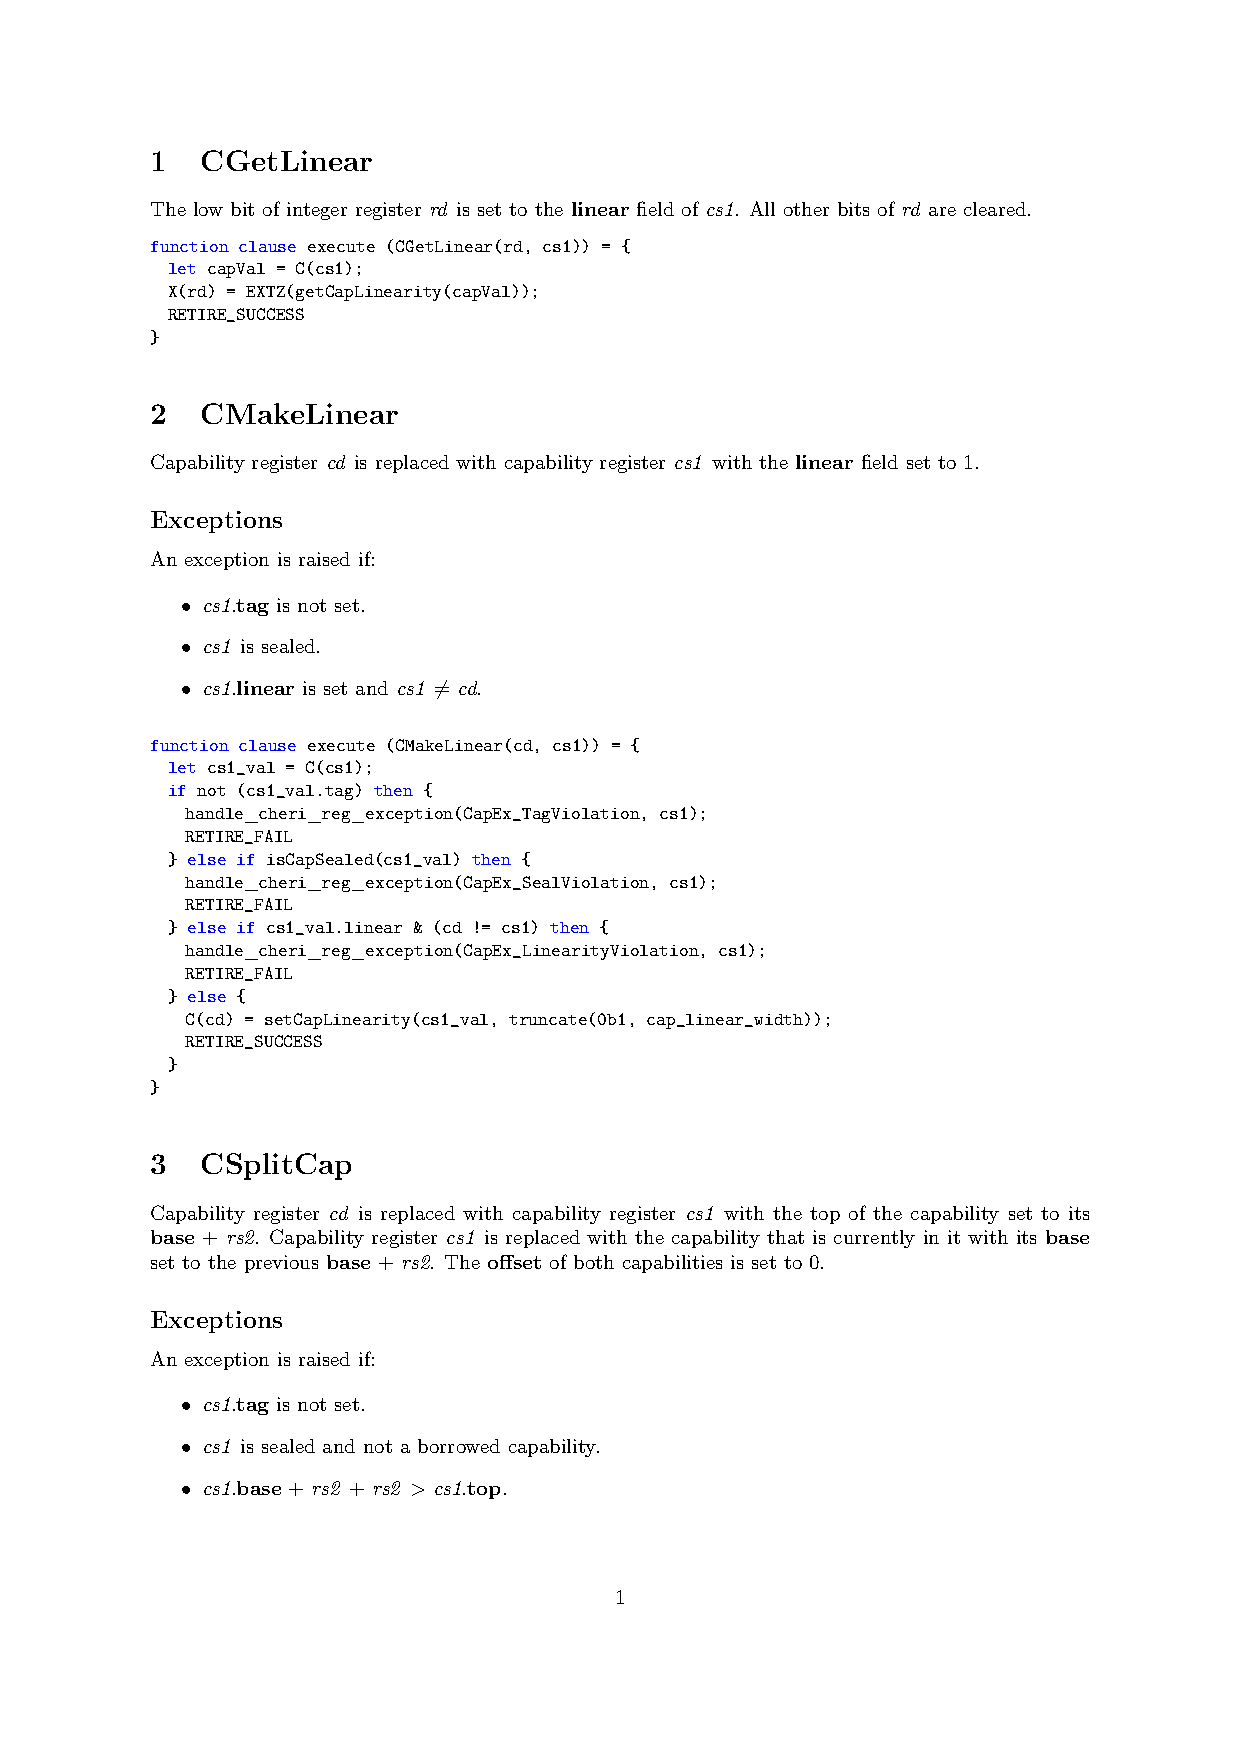
\includepdf[pages=-]{sailcode.pdf}

%%% Local Variables: 
%%% mode: latex
%%% TeX-master: "thesis"
%%% End: 

\chapter{Short Paper}
\label{app:paper}
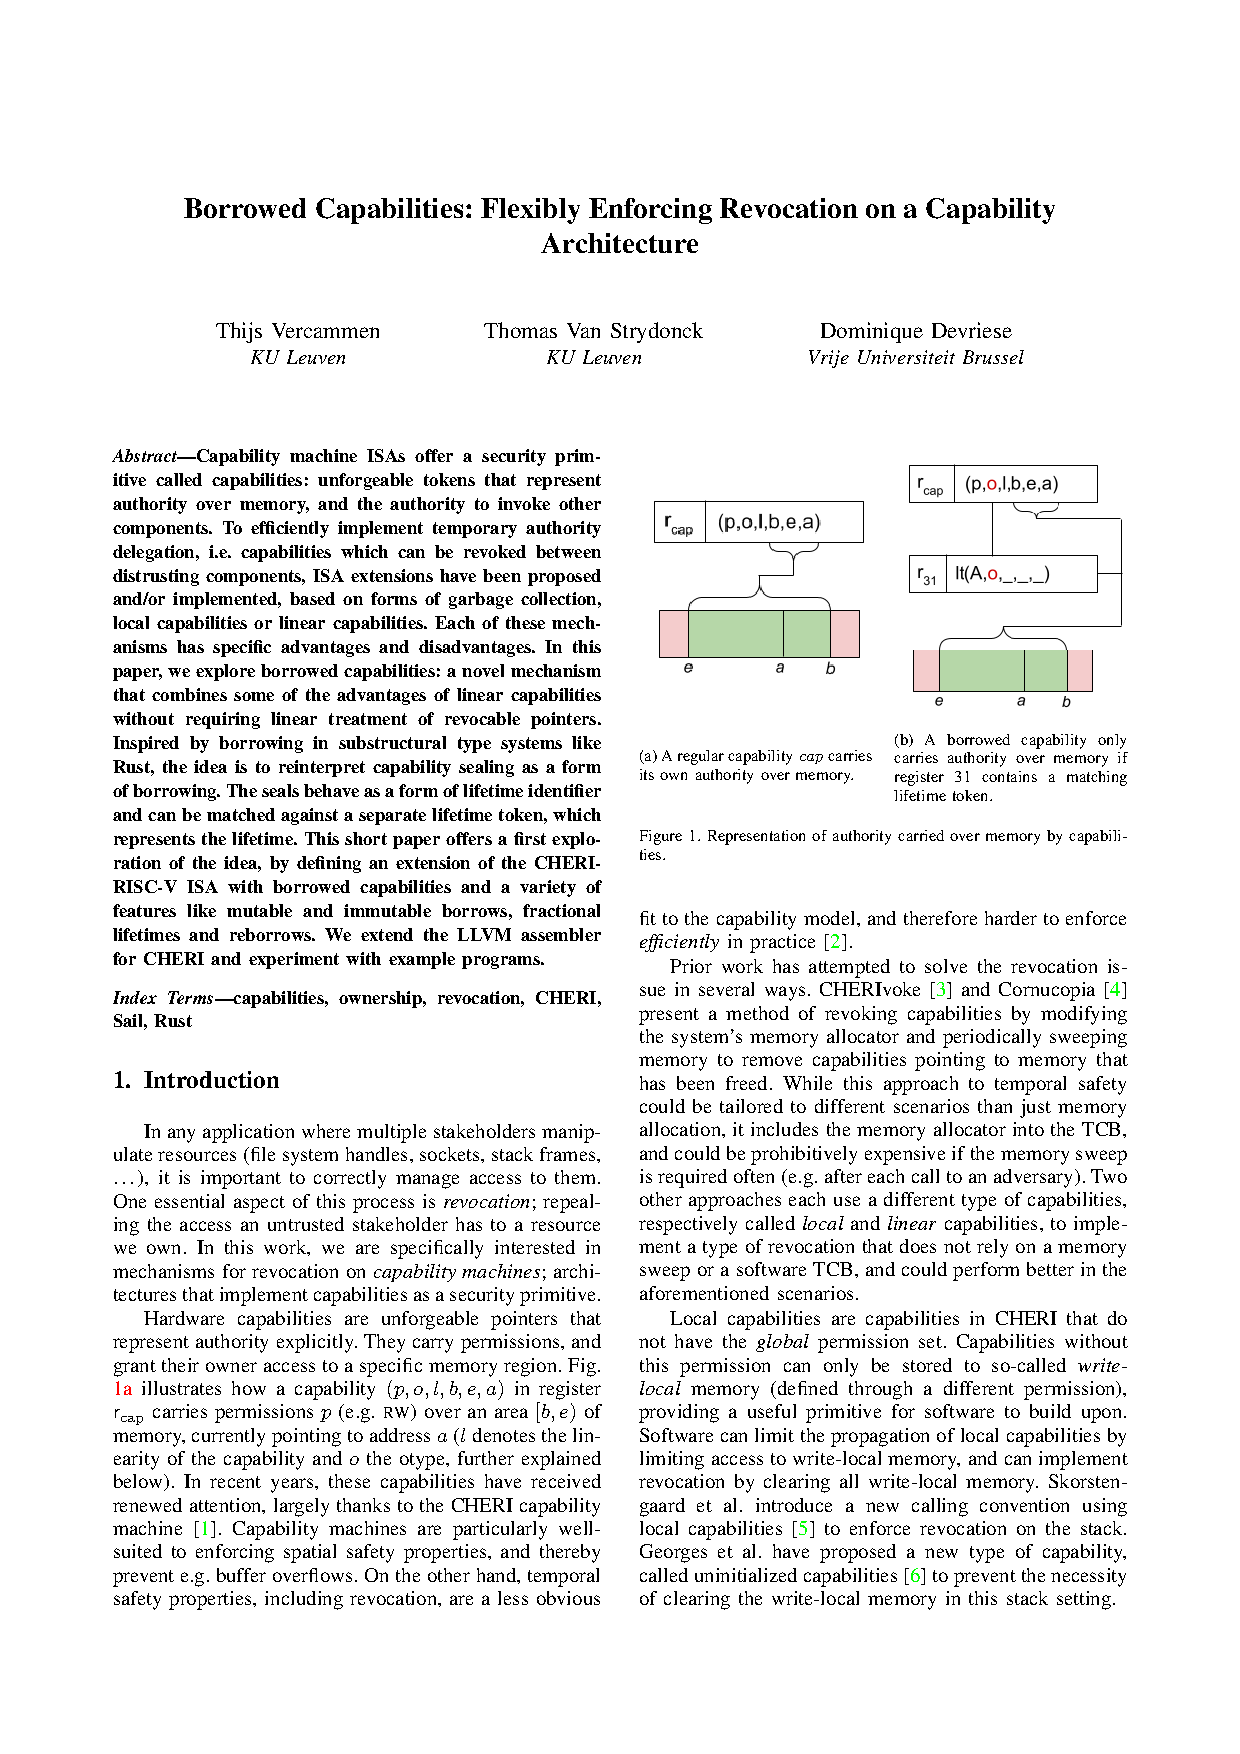
\includepdf[pages=-]{paper.pdf}

%%% Local Variables: 
%%% mode: latex
%%% TeX-master: "thesis"
%%% End: 


\backmatter
% The bibliography comes after the appendices.
% You can replace the standard "abbrv" bibliography style by another one.
\bibliographystyle{abbrv}
\bibliography{references}

\end{document}

%%% Local Variables: 
%%% mode: latex
%%% TeX-master: t
%%% End: 
